% !TeX program = pdflatex
% Отчёт по заданию 2 «Состояния космического аппарата Shuttle» (вариант 18),
% ГОСТ 7.32-2017. Все числа вставляются макросами из tables/macros.tex
% (см. src/modeling.py); ручное редактирование чисел не используется.
\documentclass[14pt,a4paper]{extarticle}

\usepackage[T2A]{fontenc}
\usepackage[utf8]{inputenc}
\usepackage[russian]{babel}
\usepackage{tempora}                % Times-подобный текстовый шрифт
\usepackage{amsmath}
\usepackage{graphicx}
\usepackage{booktabs}
\usepackage{array}
\usepackage{float}
\usepackage{setspace}
\usepackage[a4paper,top=20mm,bottom=20mm,left=30mm,right=15mm]{geometry}
\usepackage{caption}
\usepackage{titlesec}
\usepackage{lastpage}
\usepackage[unicode,hidelinks]{hyperref}

% --- Оформление по ГОСТ 7.32-2017 -----------------------------------------
\onehalfspacing
\setlength{\parindent}{12.5mm}
\setlength{\parskip}{0pt}
\setlength{\emergencystretch}{2em}
\setcounter{tocdepth}{2}

% «Рисунок N --- Название» под рисунком, «Таблица N --- Название» над таблицей
\DeclareCaptionLabelSeparator{gostdash}{ --- }
\captionsetup[table]{labelsep=gostdash,justification=raggedright,
  singlelinecheck=false,position=above,skip=6pt}
\captionsetup[figure]{labelsep=gostdash,justification=centering,
  singlelinecheck=false,position=below,skip=6pt}
\addto\captionsrussian{%
  \renewcommand{\figurename}{Рисунок}%
  \renewcommand{\tablename}{Таблица}%
}

% Заголовки разделов: с абзацного отступа, полужирные
\titleformat{\section}{\bfseries\raggedright}{\thesection}{0.6em}{}
\titleformat{\subsection}{\bfseries\raggedright}{\thesubsection}{0.6em}{}
\titlespacing*{\section}{\parindent}{14pt}{10pt}
\titlespacing*{\subsection}{\parindent}{12pt}{8pt}

% Список источников: «1.» в перечне, без собственного заголовка
\makeatletter
\renewcommand{\@biblabel}[1]{#1.}
\renewenvironment{thebibliography}[1]
     {\list{\@biblabel{\@arabic\c@enumiv}}%
           {\settowidth\labelwidth{\@biblabel{#1}}%
            \leftmargin\labelwidth
            \advance\leftmargin\labelsep
            \usecounter{enumiv}%
            \let\p@enumiv\@empty
            \renewcommand\theenumiv{\@arabic\c@enumiv}}%
      \sloppy
      \clubpenalty\@clubpenalty
      \widowpenalty4000%
      \sfcode`\.\@m}
     {\def\@noitemerr
       {\@latex@warning{Empty `thebibliography' environment}}%
      \endlist}
\makeatother
\addto\captionsrussian{%
  \renewcommand{\refname}{СПИСОК ИСПОЛЬЗОВАННЫХ ИСТОЧНИКОВ}%
}

% Содержание: заголовок по центру, список без полуторного интервала
\makeatletter
\renewcommand\tableofcontents{%
  \clearpage
  \begin{spacing}{1.0}%
  \begin{center}\bfseries СОДЕРЖАНИЕ\end{center}%
  \@starttoc{toc}%
  \end{spacing}%
}
\makeatother

% Структурный элемент: с нового листа, прописными, по центру
\newcommand{\struct}[1]{%
  \clearpage
  \begin{center}\bfseries #1\end{center}%
  \addcontentsline{toc}{section}{#1}%
}

% Автоматически сгенерировано src/modeling.py; не редактировать.

\newcommand{\NTrain}{43500}
\newcommand{\NTest}{14500}
\newcommand{\NTotal}{58000}
\newcommand{\NFeatures}{9}
\newcommand{\NClasses}{7}
\newcommand{\ShareMajorTrain}{78,41}
\newcommand{\ShareMajorTest}{79,16}
\newcommand{\ShareMinorTrain}{0,43}
\newcommand{\ShareMinorTest}{0,40}
\newcommand{\NDupTrain}{0}
\newcommand{\NDupTest}{0}
\newcommand{\NOverlap}{0}
\newcommand{\NMissing}{0}
\newcommand{\NFig}{13}
\newcommand{\NTab}{11}
\newcommand{\NSrc}{9}
\newcommand{\NApp}{2}
\newcommand{\NClassOneTrain}{34108}
\newcommand{\NClassOneTest}{11478}
\newcommand{\ShareClassOneTrain}{78,41}
\newcommand{\ShareClassOneTest}{79,16}
\newcommand{\NClassTwoTrain}{37}
\newcommand{\NClassTwoTest}{13}
\newcommand{\ShareClassTwoTrain}{0,09}
\newcommand{\ShareClassTwoTest}{0,09}
\newcommand{\NClassThreeTrain}{132}
\newcommand{\NClassThreeTest}{39}
\newcommand{\ShareClassThreeTrain}{0,30}
\newcommand{\ShareClassThreeTest}{0,27}
\newcommand{\NClassFourTrain}{6748}
\newcommand{\NClassFourTest}{2155}
\newcommand{\ShareClassFourTrain}{15,51}
\newcommand{\ShareClassFourTest}{14,86}
\newcommand{\NClassFiveTrain}{2458}
\newcommand{\NClassFiveTest}{809}
\newcommand{\ShareClassFiveTrain}{5,65}
\newcommand{\ShareClassFiveTest}{5,58}
\newcommand{\NClassSixTrain}{6}
\newcommand{\NClassSixTest}{4}
\newcommand{\ShareClassSixTrain}{0,01}
\newcommand{\ShareClassSixTest}{0,03}
\newcommand{\NClassSevenTrain}{11}
\newcommand{\NClassSevenTest}{2}
\newcommand{\ShareClassSevenTrain}{0,03}
\newcommand{\ShareClassSevenTest}{0,01}
\newcommand{\CvFDummy}{0,13}
\newcommand{\CvFDummyStd}{0,00}
\newcommand{\AccDummy}{0,7916}
\newcommand{\BalDummy}{0,14}
\newcommand{\FOneDummy}{0,13}
\newcommand{\WfDummy}{0,70}
\newcommand{\AucDummy}{0,50}
\newcommand{\ParamsDummy}{---}
\newcommand{\CvFLogreg}{0,86}
\newcommand{\CvFLogregStd}{0,05}
\newcommand{\AccLogreg}{0,9539}
\newcommand{\BalLogreg}{0,99}
\newcommand{\FOneLogreg}{0,82}
\newcommand{\WfLogreg}{0,96}
\newcommand{\AucLogreg}{1,00}
\newcommand{\ParamsLogreg}{C=1, class\_weight=balanced}
\newcommand{\CvFKnn}{0,93}
\newcommand{\CvFKnnStd}{0,02}
\newcommand{\AccKnn}{0,9991}
\newcommand{\BalKnn}{0,87}
\newcommand{\FOneKnn}{0,88}
\newcommand{\WfKnn}{1,00}
\newcommand{\AucKnn}{0,93}
\newcommand{\ParamsKnn}{n\_neighbors=1, weights=uniform}
\newcommand{\CvFSvm}{0,91}
\newcommand{\CvFSvmStd}{0,02}
\newcommand{\AccSvm}{0,9976}
\newcommand{\BalSvm}{0,91}
\newcommand{\FOneSvm}{0,84}
\newcommand{\WfSvm}{1,00}
\newcommand{\AucSvm}{1,00}
\newcommand{\ParamsSvm}{C=100, class\_weight=balanced, gamma=0,01}
\newcommand{\CvFTree}{0,95}
\newcommand{\CvFTreeStd}{0,07}
\newcommand{\AccTree}{0,9999}
\newcommand{\BalTree}{0,99}
\newcommand{\FOneTree}{0,99}
\newcommand{\WfTree}{1,00}
\newcommand{\AucTree}{0,99}
\newcommand{\ParamsTree}{max\_depth=10, min\_samples\_leaf=1}
\newcommand{\CvFRf}{0,94}
\newcommand{\CvFRfStd}{0,08}
\newcommand{\AccRf}{0,9999}
\newcommand{\BalRf}{0,99}
\newcommand{\FOneRf}{0,99}
\newcommand{\WfRf}{1,00}
\newcommand{\AucRf}{1,00}
\newcommand{\ParamsRf}{max\_depth=10, max\_features=0,5, min\_samples\_leaf=1, n\_estimators=200}
\newcommand{\CvFHgb}{0,96}
\newcommand{\CvFHgbStd}{0,06}
\newcommand{\AccHgb}{0,9999}
\newcommand{\BalHgb}{0,99}
\newcommand{\FOneHgb}{0,99}
\newcommand{\WfHgb}{1,00}
\newcommand{\AucHgb}{1,00}
\newcommand{\ParamsHgb}{class\_weight=balanced, l2\_regularization=0, learning\_rate=0,056, max\_iter=100, max\_leaf\_nodes=31, min\_samples\_leaf=10}
\newcommand{\BestName}{Градиентный бустинг (HistGB)}
\newcommand{\BestCvF}{0,96}
\newcommand{\BestCvFStd}{0,06}
\newcommand{\BestAcc}{0,9999}
\newcommand{\BestBal}{0,99}
\newcommand{\BestFOne}{0,99}
\newcommand{\BestWf}{1,00}
\newcommand{\BestAuc}{1,00}
\newcommand{\BestParams}{class\_weight=balanced, l2\_regularization=0, learning\_rate=0,056, max\_iter=100, max\_leaf\_nodes=31, min\_samples\_leaf=10}
\newcommand{\PrecClassOne}{1,00}
\newcommand{\RecClassOne}{1,00}
\newcommand{\FOneClassOne}{1,00}
\newcommand{\SupportClassOne}{11478}
\newcommand{\AucClassOne}{1,00}
\newcommand{\PrecClassTwo}{1,00}
\newcommand{\RecClassTwo}{0,92}
\newcommand{\FOneClassTwo}{0,96}
\newcommand{\SupportClassTwo}{13}
\newcommand{\AucClassTwo}{1,00}
\newcommand{\PrecClassThree}{1,00}
\newcommand{\RecClassThree}{1,00}
\newcommand{\FOneClassThree}{1,00}
\newcommand{\SupportClassThree}{39}
\newcommand{\AucClassThree}{1,00}
\newcommand{\PrecClassFour}{1,00}
\newcommand{\RecClassFour}{1,00}
\newcommand{\FOneClassFour}{1,00}
\newcommand{\SupportClassFour}{2155}
\newcommand{\AucClassFour}{1,00}
\newcommand{\PrecClassFive}{1,00}
\newcommand{\RecClassFive}{1,00}
\newcommand{\FOneClassFive}{1,00}
\newcommand{\SupportClassFive}{809}
\newcommand{\AucClassFive}{1,00}
\newcommand{\PrecClassSix}{1,00}
\newcommand{\RecClassSix}{1,00}
\newcommand{\FOneClassSix}{1,00}
\newcommand{\SupportClassSix}{4}
\newcommand{\AucClassSix}{1,00}
\newcommand{\PrecClassSeven}{1,00}
\newcommand{\RecClassSeven}{1,00}
\newcommand{\FOneClassSeven}{1,00}
\newcommand{\SupportClassSeven}{2}
\newcommand{\AucClassSeven}{1,00}
\newcommand{\PrecDummyClassOne}{0,79}
\newcommand{\RecDummyClassOne}{1,00}
\newcommand{\FOneDummyClassOne}{0,88}
\newcommand{\PrecDummyClassTwo}{0,00}
\newcommand{\RecDummyClassTwo}{0,00}
\newcommand{\FOneDummyClassTwo}{0,00}
\newcommand{\PrecDummyClassThree}{0,00}
\newcommand{\RecDummyClassThree}{0,00}
\newcommand{\FOneDummyClassThree}{0,00}
\newcommand{\PrecDummyClassFour}{0,00}
\newcommand{\RecDummyClassFour}{0,00}
\newcommand{\FOneDummyClassFour}{0,00}
\newcommand{\PrecDummyClassFive}{0,00}
\newcommand{\RecDummyClassFive}{0,00}
\newcommand{\FOneDummyClassFive}{0,00}
\newcommand{\PrecDummyClassSix}{0,00}
\newcommand{\RecDummyClassSix}{0,00}
\newcommand{\FOneDummyClassSix}{0,00}
\newcommand{\PrecDummyClassSeven}{0,00}
\newcommand{\RecDummyClassSeven}{0,00}
\newcommand{\FOneDummyClassSeven}{0,00}
\newcommand{\PrecLogregClassOne}{1,00}
\newcommand{\RecLogregClassOne}{0,94}
\newcommand{\FOneLogregClassOne}{0,97}
\newcommand{\PrecLogregClassTwo}{0,62}
\newcommand{\RecLogregClassTwo}{1,00}
\newcommand{\FOneLogregClassTwo}{0,76}
\newcommand{\PrecLogregClassThree}{0,74}
\newcommand{\RecLogregClassThree}{1,00}
\newcommand{\FOneLogregClassThree}{0,85}
\newcommand{\PrecLogregClassFour}{0,77}
\newcommand{\RecLogregClassFour}{1,00}
\newcommand{\FOneLogregClassFour}{0,87}
\newcommand{\PrecLogregClassFive}{1,00}
\newcommand{\RecLogregClassFive}{1,00}
\newcommand{\FOneLogregClassFive}{1,00}
\newcommand{\PrecLogregClassSix}{0,57}
\newcommand{\RecLogregClassSix}{1,00}
\newcommand{\FOneLogregClassSix}{0,73}
\newcommand{\PrecLogregClassSeven}{0,40}
\newcommand{\RecLogregClassSeven}{1,00}
\newcommand{\FOneLogregClassSeven}{0,57}
\newcommand{\PrecKnnClassOne}{1,00}
\newcommand{\RecKnnClassOne}{1,00}
\newcommand{\FOneKnnClassOne}{1,00}
\newcommand{\PrecKnnClassTwo}{1,00}
\newcommand{\RecKnnClassTwo}{0,92}
\newcommand{\FOneKnnClassTwo}{0,96}
\newcommand{\PrecKnnClassThree}{0,95}
\newcommand{\RecKnnClassThree}{0,90}
\newcommand{\FOneKnnClassThree}{0,92}
\newcommand{\PrecKnnClassFour}{1,00}
\newcommand{\RecKnnClassFour}{1,00}
\newcommand{\FOneKnnClassFour}{1,00}
\newcommand{\PrecKnnClassFive}{1,00}
\newcommand{\RecKnnClassFive}{1,00}
\newcommand{\FOneKnnClassFive}{1,00}
\newcommand{\PrecKnnClassSix}{1,00}
\newcommand{\RecKnnClassSix}{0,75}
\newcommand{\FOneKnnClassSix}{0,86}
\newcommand{\PrecKnnClassSeven}{0,33}
\newcommand{\RecKnnClassSeven}{0,50}
\newcommand{\FOneKnnClassSeven}{0,40}
\newcommand{\PrecSvmClassOne}{1,00}
\newcommand{\RecSvmClassOne}{1,00}
\newcommand{\FOneSvmClassOne}{1,00}
\newcommand{\PrecSvmClassTwo}{0,75}
\newcommand{\RecSvmClassTwo}{0,92}
\newcommand{\FOneSvmClassTwo}{0,83}
\newcommand{\PrecSvmClassThree}{0,61}
\newcommand{\RecSvmClassThree}{0,97}
\newcommand{\FOneSvmClassThree}{0,75}
\newcommand{\PrecSvmClassFour}{1,00}
\newcommand{\RecSvmClassFour}{1,00}
\newcommand{\FOneSvmClassFour}{1,00}
\newcommand{\PrecSvmClassFive}{1,00}
\newcommand{\RecSvmClassFive}{1,00}
\newcommand{\FOneSvmClassFive}{1,00}
\newcommand{\PrecSvmClassSix}{1,00}
\newcommand{\RecSvmClassSix}{0,50}
\newcommand{\FOneSvmClassSix}{0,67}
\newcommand{\PrecSvmClassSeven}{0,50}
\newcommand{\RecSvmClassSeven}{1,00}
\newcommand{\FOneSvmClassSeven}{0,67}
\newcommand{\PrecTreeClassOne}{1,00}
\newcommand{\RecTreeClassOne}{1,00}
\newcommand{\FOneTreeClassOne}{1,00}
\newcommand{\PrecTreeClassTwo}{1,00}
\newcommand{\RecTreeClassTwo}{0,92}
\newcommand{\FOneTreeClassTwo}{0,96}
\newcommand{\PrecTreeClassThree}{0,97}
\newcommand{\RecTreeClassThree}{1,00}
\newcommand{\FOneTreeClassThree}{0,99}
\newcommand{\PrecTreeClassFour}{1,00}
\newcommand{\RecTreeClassFour}{1,00}
\newcommand{\FOneTreeClassFour}{1,00}
\newcommand{\PrecTreeClassFive}{1,00}
\newcommand{\RecTreeClassFive}{1,00}
\newcommand{\FOneTreeClassFive}{1,00}
\newcommand{\PrecTreeClassSix}{1,00}
\newcommand{\RecTreeClassSix}{1,00}
\newcommand{\FOneTreeClassSix}{1,00}
\newcommand{\PrecTreeClassSeven}{1,00}
\newcommand{\RecTreeClassSeven}{1,00}
\newcommand{\FOneTreeClassSeven}{1,00}
\newcommand{\PrecRfClassOne}{1,00}
\newcommand{\RecRfClassOne}{1,00}
\newcommand{\FOneRfClassOne}{1,00}
\newcommand{\PrecRfClassTwo}{1,00}
\newcommand{\RecRfClassTwo}{0,92}
\newcommand{\FOneRfClassTwo}{0,96}
\newcommand{\PrecRfClassThree}{1,00}
\newcommand{\RecRfClassThree}{1,00}
\newcommand{\FOneRfClassThree}{1,00}
\newcommand{\PrecRfClassFour}{1,00}
\newcommand{\RecRfClassFour}{1,00}
\newcommand{\FOneRfClassFour}{1,00}
\newcommand{\PrecRfClassFive}{1,00}
\newcommand{\RecRfClassFive}{1,00}
\newcommand{\FOneRfClassFive}{1,00}
\newcommand{\PrecRfClassSix}{1,00}
\newcommand{\RecRfClassSix}{1,00}
\newcommand{\FOneRfClassSix}{1,00}
\newcommand{\PrecRfClassSeven}{1,00}
\newcommand{\RecRfClassSeven}{1,00}
\newcommand{\FOneRfClassSeven}{1,00}
\newcommand{\PrecHgbClassOne}{1,00}
\newcommand{\RecHgbClassOne}{1,00}
\newcommand{\FOneHgbClassOne}{1,00}
\newcommand{\PrecHgbClassTwo}{1,00}
\newcommand{\RecHgbClassTwo}{0,92}
\newcommand{\FOneHgbClassTwo}{0,96}
\newcommand{\PrecHgbClassThree}{1,00}
\newcommand{\RecHgbClassThree}{1,00}
\newcommand{\FOneHgbClassThree}{1,00}
\newcommand{\PrecHgbClassFour}{1,00}
\newcommand{\RecHgbClassFour}{1,00}
\newcommand{\FOneHgbClassFour}{1,00}
\newcommand{\PrecHgbClassFive}{1,00}
\newcommand{\RecHgbClassFive}{1,00}
\newcommand{\FOneHgbClassFive}{1,00}
\newcommand{\PrecHgbClassSix}{1,00}
\newcommand{\RecHgbClassSix}{1,00}
\newcommand{\FOneHgbClassSix}{1,00}
\newcommand{\PrecHgbClassSeven}{1,00}
\newcommand{\RecHgbClassSeven}{1,00}
\newcommand{\FOneHgbClassSeven}{1,00}
\newcommand{\ConfOneOne}{1,00}
\newcommand{\ConfOneTwo}{0,00}
\newcommand{\ConfOneThree}{0,00}
\newcommand{\ConfOneFour}{0,00}
\newcommand{\ConfOneFive}{0,00}
\newcommand{\ConfOneSix}{0,00}
\newcommand{\ConfOneSeven}{0,00}
\newcommand{\ConfTwoOne}{0,00}
\newcommand{\ConfTwoTwo}{0,92}
\newcommand{\ConfTwoThree}{0,00}
\newcommand{\ConfTwoFour}{0,08}
\newcommand{\ConfTwoFive}{0,00}
\newcommand{\ConfTwoSix}{0,00}
\newcommand{\ConfTwoSeven}{0,00}
\newcommand{\ConfThreeOne}{0,00}
\newcommand{\ConfThreeTwo}{0,00}
\newcommand{\ConfThreeThree}{1,00}
\newcommand{\ConfThreeFour}{0,00}
\newcommand{\ConfThreeFive}{0,00}
\newcommand{\ConfThreeSix}{0,00}
\newcommand{\ConfThreeSeven}{0,00}
\newcommand{\ConfFourOne}{0,00}
\newcommand{\ConfFourTwo}{0,00}
\newcommand{\ConfFourThree}{0,00}
\newcommand{\ConfFourFour}{1,00}
\newcommand{\ConfFourFive}{0,00}
\newcommand{\ConfFourSix}{0,00}
\newcommand{\ConfFourSeven}{0,00}
\newcommand{\ConfFiveOne}{0,00}
\newcommand{\ConfFiveTwo}{0,00}
\newcommand{\ConfFiveThree}{0,00}
\newcommand{\ConfFiveFour}{0,00}
\newcommand{\ConfFiveFive}{1,00}
\newcommand{\ConfFiveSix}{0,00}
\newcommand{\ConfFiveSeven}{0,00}
\newcommand{\ConfSixOne}{0,00}
\newcommand{\ConfSixTwo}{0,00}
\newcommand{\ConfSixThree}{0,00}
\newcommand{\ConfSixFour}{0,00}
\newcommand{\ConfSixFive}{0,00}
\newcommand{\ConfSixSix}{1,00}
\newcommand{\ConfSixSeven}{0,00}
\newcommand{\ConfSevenOne}{0,00}
\newcommand{\ConfSevenTwo}{0,00}
\newcommand{\ConfSevenThree}{0,00}
\newcommand{\ConfSevenFour}{0,00}
\newcommand{\ConfSevenFive}{0,00}
\newcommand{\ConfSevenSix}{0,00}
\newcommand{\ConfSevenSeven}{1,00}
\newcommand{\ConfCntOneOne}{11477}
\newcommand{\ConfCntOneTwo}{0}
\newcommand{\ConfCntOneThree}{0}
\newcommand{\ConfCntOneFour}{0}
\newcommand{\ConfCntOneFive}{1}
\newcommand{\ConfCntOneSix}{0}
\newcommand{\ConfCntOneSeven}{0}
\newcommand{\ConfCntTwoOne}{0}
\newcommand{\ConfCntTwoTwo}{12}
\newcommand{\ConfCntTwoThree}{0}
\newcommand{\ConfCntTwoFour}{1}
\newcommand{\ConfCntTwoFive}{0}
\newcommand{\ConfCntTwoSix}{0}
\newcommand{\ConfCntTwoSeven}{0}
\newcommand{\ConfCntThreeOne}{0}
\newcommand{\ConfCntThreeTwo}{0}
\newcommand{\ConfCntThreeThree}{39}
\newcommand{\ConfCntThreeFour}{0}
\newcommand{\ConfCntThreeFive}{0}
\newcommand{\ConfCntThreeSix}{0}
\newcommand{\ConfCntThreeSeven}{0}
\newcommand{\ConfCntFourOne}{0}
\newcommand{\ConfCntFourTwo}{0}
\newcommand{\ConfCntFourThree}{0}
\newcommand{\ConfCntFourFour}{2155}
\newcommand{\ConfCntFourFive}{0}
\newcommand{\ConfCntFourSix}{0}
\newcommand{\ConfCntFourSeven}{0}
\newcommand{\ConfCntFiveOne}{0}
\newcommand{\ConfCntFiveTwo}{0}
\newcommand{\ConfCntFiveThree}{0}
\newcommand{\ConfCntFiveFour}{0}
\newcommand{\ConfCntFiveFive}{809}
\newcommand{\ConfCntFiveSix}{0}
\newcommand{\ConfCntFiveSeven}{0}
\newcommand{\ConfCntSixOne}{0}
\newcommand{\ConfCntSixTwo}{0}
\newcommand{\ConfCntSixThree}{0}
\newcommand{\ConfCntSixFour}{0}
\newcommand{\ConfCntSixFive}{0}
\newcommand{\ConfCntSixSix}{4}
\newcommand{\ConfCntSixSeven}{0}
\newcommand{\ConfCntSevenOne}{0}
\newcommand{\ConfCntSevenTwo}{0}
\newcommand{\ConfCntSevenThree}{0}
\newcommand{\ConfCntSevenFour}{0}
\newcommand{\ConfCntSevenFive}{0}
\newcommand{\ConfCntSevenSix}{0}
\newcommand{\ConfCntSevenSeven}{2}
\newcommand{\ConfDummyOneOne}{1,00}
\newcommand{\ConfCntDummyOneOne}{11478}
\newcommand{\ConfDummyOneTwo}{0,00}
\newcommand{\ConfCntDummyOneTwo}{0}
\newcommand{\ConfDummyOneThree}{0,00}
\newcommand{\ConfCntDummyOneThree}{0}
\newcommand{\ConfDummyOneFour}{0,00}
\newcommand{\ConfCntDummyOneFour}{0}
\newcommand{\ConfDummyOneFive}{0,00}
\newcommand{\ConfCntDummyOneFive}{0}
\newcommand{\ConfDummyOneSix}{0,00}
\newcommand{\ConfCntDummyOneSix}{0}
\newcommand{\ConfDummyOneSeven}{0,00}
\newcommand{\ConfCntDummyOneSeven}{0}
\newcommand{\ConfDummyTwoOne}{1,00}
\newcommand{\ConfCntDummyTwoOne}{13}
\newcommand{\ConfDummyTwoTwo}{0,00}
\newcommand{\ConfCntDummyTwoTwo}{0}
\newcommand{\ConfDummyTwoThree}{0,00}
\newcommand{\ConfCntDummyTwoThree}{0}
\newcommand{\ConfDummyTwoFour}{0,00}
\newcommand{\ConfCntDummyTwoFour}{0}
\newcommand{\ConfDummyTwoFive}{0,00}
\newcommand{\ConfCntDummyTwoFive}{0}
\newcommand{\ConfDummyTwoSix}{0,00}
\newcommand{\ConfCntDummyTwoSix}{0}
\newcommand{\ConfDummyTwoSeven}{0,00}
\newcommand{\ConfCntDummyTwoSeven}{0}
\newcommand{\ConfDummyThreeOne}{1,00}
\newcommand{\ConfCntDummyThreeOne}{39}
\newcommand{\ConfDummyThreeTwo}{0,00}
\newcommand{\ConfCntDummyThreeTwo}{0}
\newcommand{\ConfDummyThreeThree}{0,00}
\newcommand{\ConfCntDummyThreeThree}{0}
\newcommand{\ConfDummyThreeFour}{0,00}
\newcommand{\ConfCntDummyThreeFour}{0}
\newcommand{\ConfDummyThreeFive}{0,00}
\newcommand{\ConfCntDummyThreeFive}{0}
\newcommand{\ConfDummyThreeSix}{0,00}
\newcommand{\ConfCntDummyThreeSix}{0}
\newcommand{\ConfDummyThreeSeven}{0,00}
\newcommand{\ConfCntDummyThreeSeven}{0}
\newcommand{\ConfDummyFourOne}{1,00}
\newcommand{\ConfCntDummyFourOne}{2155}
\newcommand{\ConfDummyFourTwo}{0,00}
\newcommand{\ConfCntDummyFourTwo}{0}
\newcommand{\ConfDummyFourThree}{0,00}
\newcommand{\ConfCntDummyFourThree}{0}
\newcommand{\ConfDummyFourFour}{0,00}
\newcommand{\ConfCntDummyFourFour}{0}
\newcommand{\ConfDummyFourFive}{0,00}
\newcommand{\ConfCntDummyFourFive}{0}
\newcommand{\ConfDummyFourSix}{0,00}
\newcommand{\ConfCntDummyFourSix}{0}
\newcommand{\ConfDummyFourSeven}{0,00}
\newcommand{\ConfCntDummyFourSeven}{0}
\newcommand{\ConfDummyFiveOne}{1,00}
\newcommand{\ConfCntDummyFiveOne}{809}
\newcommand{\ConfDummyFiveTwo}{0,00}
\newcommand{\ConfCntDummyFiveTwo}{0}
\newcommand{\ConfDummyFiveThree}{0,00}
\newcommand{\ConfCntDummyFiveThree}{0}
\newcommand{\ConfDummyFiveFour}{0,00}
\newcommand{\ConfCntDummyFiveFour}{0}
\newcommand{\ConfDummyFiveFive}{0,00}
\newcommand{\ConfCntDummyFiveFive}{0}
\newcommand{\ConfDummyFiveSix}{0,00}
\newcommand{\ConfCntDummyFiveSix}{0}
\newcommand{\ConfDummyFiveSeven}{0,00}
\newcommand{\ConfCntDummyFiveSeven}{0}
\newcommand{\ConfDummySixOne}{1,00}
\newcommand{\ConfCntDummySixOne}{4}
\newcommand{\ConfDummySixTwo}{0,00}
\newcommand{\ConfCntDummySixTwo}{0}
\newcommand{\ConfDummySixThree}{0,00}
\newcommand{\ConfCntDummySixThree}{0}
\newcommand{\ConfDummySixFour}{0,00}
\newcommand{\ConfCntDummySixFour}{0}
\newcommand{\ConfDummySixFive}{0,00}
\newcommand{\ConfCntDummySixFive}{0}
\newcommand{\ConfDummySixSix}{0,00}
\newcommand{\ConfCntDummySixSix}{0}
\newcommand{\ConfDummySixSeven}{0,00}
\newcommand{\ConfCntDummySixSeven}{0}
\newcommand{\ConfDummySevenOne}{1,00}
\newcommand{\ConfCntDummySevenOne}{2}
\newcommand{\ConfDummySevenTwo}{0,00}
\newcommand{\ConfCntDummySevenTwo}{0}
\newcommand{\ConfDummySevenThree}{0,00}
\newcommand{\ConfCntDummySevenThree}{0}
\newcommand{\ConfDummySevenFour}{0,00}
\newcommand{\ConfCntDummySevenFour}{0}
\newcommand{\ConfDummySevenFive}{0,00}
\newcommand{\ConfCntDummySevenFive}{0}
\newcommand{\ConfDummySevenSix}{0,00}
\newcommand{\ConfCntDummySevenSix}{0}
\newcommand{\ConfDummySevenSeven}{0,00}
\newcommand{\ConfCntDummySevenSeven}{0}
\newcommand{\ConfLogregOneOne}{0,94}
\newcommand{\ConfCntLogregOneOne}{10815}
\newcommand{\ConfLogregOneTwo}{0,00}
\newcommand{\ConfCntLogregOneTwo}{7}
\newcommand{\ConfLogregOneThree}{0,00}
\newcommand{\ConfCntLogregOneThree}{13}
\newcommand{\ConfLogregOneFour}{0,06}
\newcommand{\ConfCntLogregOneFour}{640}
\newcommand{\ConfLogregOneFive}{0,00}
\newcommand{\ConfCntLogregOneFive}{0}
\newcommand{\ConfLogregOneSix}{0,00}
\newcommand{\ConfCntLogregOneSix}{0}
\newcommand{\ConfLogregOneSeven}{0,00}
\newcommand{\ConfCntLogregOneSeven}{3}
\newcommand{\ConfLogregTwoOne}{0,00}
\newcommand{\ConfCntLogregTwoOne}{0}
\newcommand{\ConfLogregTwoTwo}{1,00}
\newcommand{\ConfCntLogregTwoTwo}{13}
\newcommand{\ConfLogregTwoThree}{0,00}
\newcommand{\ConfCntLogregTwoThree}{0}
\newcommand{\ConfLogregTwoFour}{0,00}
\newcommand{\ConfCntLogregTwoFour}{0}
\newcommand{\ConfLogregTwoFive}{0,00}
\newcommand{\ConfCntLogregTwoFive}{0}
\newcommand{\ConfLogregTwoSix}{0,00}
\newcommand{\ConfCntLogregTwoSix}{0}
\newcommand{\ConfLogregTwoSeven}{0,00}
\newcommand{\ConfCntLogregTwoSeven}{0}
\newcommand{\ConfLogregThreeOne}{0,00}
\newcommand{\ConfCntLogregThreeOne}{0}
\newcommand{\ConfLogregThreeTwo}{0,00}
\newcommand{\ConfCntLogregThreeTwo}{0}
\newcommand{\ConfLogregThreeThree}{1,00}
\newcommand{\ConfCntLogregThreeThree}{39}
\newcommand{\ConfLogregThreeFour}{0,00}
\newcommand{\ConfCntLogregThreeFour}{0}
\newcommand{\ConfLogregThreeFive}{0,00}
\newcommand{\ConfCntLogregThreeFive}{0}
\newcommand{\ConfLogregThreeSix}{0,00}
\newcommand{\ConfCntLogregThreeSix}{0}
\newcommand{\ConfLogregThreeSeven}{0,00}
\newcommand{\ConfCntLogregThreeSeven}{0}
\newcommand{\ConfLogregFourOne}{0,00}
\newcommand{\ConfCntLogregFourOne}{0}
\newcommand{\ConfLogregFourTwo}{0,00}
\newcommand{\ConfCntLogregFourTwo}{1}
\newcommand{\ConfLogregFourThree}{0,00}
\newcommand{\ConfCntLogregFourThree}{1}
\newcommand{\ConfLogregFourFour}{1,00}
\newcommand{\ConfCntLogregFourFour}{2153}
\newcommand{\ConfLogregFourFive}{0,00}
\newcommand{\ConfCntLogregFourFive}{0}
\newcommand{\ConfLogregFourSix}{0,00}
\newcommand{\ConfCntLogregFourSix}{0}
\newcommand{\ConfLogregFourSeven}{0,00}
\newcommand{\ConfCntLogregFourSeven}{0}
\newcommand{\ConfLogregFiveOne}{0,00}
\newcommand{\ConfCntLogregFiveOne}{0}
\newcommand{\ConfLogregFiveTwo}{0,00}
\newcommand{\ConfCntLogregFiveTwo}{0}
\newcommand{\ConfLogregFiveThree}{0,00}
\newcommand{\ConfCntLogregFiveThree}{0}
\newcommand{\ConfLogregFiveFour}{0,00}
\newcommand{\ConfCntLogregFiveFour}{0}
\newcommand{\ConfLogregFiveFive}{1,00}
\newcommand{\ConfCntLogregFiveFive}{806}
\newcommand{\ConfLogregFiveSix}{0,00}
\newcommand{\ConfCntLogregFiveSix}{3}
\newcommand{\ConfLogregFiveSeven}{0,00}
\newcommand{\ConfCntLogregFiveSeven}{0}
\newcommand{\ConfLogregSixOne}{0,00}
\newcommand{\ConfCntLogregSixOne}{0}
\newcommand{\ConfLogregSixTwo}{0,00}
\newcommand{\ConfCntLogregSixTwo}{0}
\newcommand{\ConfLogregSixThree}{0,00}
\newcommand{\ConfCntLogregSixThree}{0}
\newcommand{\ConfLogregSixFour}{0,00}
\newcommand{\ConfCntLogregSixFour}{0}
\newcommand{\ConfLogregSixFive}{0,00}
\newcommand{\ConfCntLogregSixFive}{0}
\newcommand{\ConfLogregSixSix}{1,00}
\newcommand{\ConfCntLogregSixSix}{4}
\newcommand{\ConfLogregSixSeven}{0,00}
\newcommand{\ConfCntLogregSixSeven}{0}
\newcommand{\ConfLogregSevenOne}{0,00}
\newcommand{\ConfCntLogregSevenOne}{0}
\newcommand{\ConfLogregSevenTwo}{0,00}
\newcommand{\ConfCntLogregSevenTwo}{0}
\newcommand{\ConfLogregSevenThree}{0,00}
\newcommand{\ConfCntLogregSevenThree}{0}
\newcommand{\ConfLogregSevenFour}{0,00}
\newcommand{\ConfCntLogregSevenFour}{0}
\newcommand{\ConfLogregSevenFive}{0,00}
\newcommand{\ConfCntLogregSevenFive}{0}
\newcommand{\ConfLogregSevenSix}{0,00}
\newcommand{\ConfCntLogregSevenSix}{0}
\newcommand{\ConfLogregSevenSeven}{1,00}
\newcommand{\ConfCntLogregSevenSeven}{2}
\newcommand{\ConfKnnOneOne}{1,00}
\newcommand{\ConfCntKnnOneOne}{11473}
\newcommand{\ConfKnnOneTwo}{0,00}
\newcommand{\ConfCntKnnOneTwo}{0}
\newcommand{\ConfKnnOneThree}{0,00}
\newcommand{\ConfCntKnnOneThree}{2}
\newcommand{\ConfKnnOneFour}{0,00}
\newcommand{\ConfCntKnnOneFour}{1}
\newcommand{\ConfKnnOneFive}{0,00}
\newcommand{\ConfCntKnnOneFive}{0}
\newcommand{\ConfKnnOneSix}{0,00}
\newcommand{\ConfCntKnnOneSix}{0}
\newcommand{\ConfKnnOneSeven}{0,00}
\newcommand{\ConfCntKnnOneSeven}{2}
\newcommand{\ConfKnnTwoOne}{0,00}
\newcommand{\ConfCntKnnTwoOne}{0}
\newcommand{\ConfKnnTwoTwo}{0,92}
\newcommand{\ConfCntKnnTwoTwo}{12}
\newcommand{\ConfKnnTwoThree}{0,00}
\newcommand{\ConfCntKnnTwoThree}{0}
\newcommand{\ConfKnnTwoFour}{0,08}
\newcommand{\ConfCntKnnTwoFour}{1}
\newcommand{\ConfKnnTwoFive}{0,00}
\newcommand{\ConfCntKnnTwoFive}{0}
\newcommand{\ConfKnnTwoSix}{0,00}
\newcommand{\ConfCntKnnTwoSix}{0}
\newcommand{\ConfKnnTwoSeven}{0,00}
\newcommand{\ConfCntKnnTwoSeven}{0}
\newcommand{\ConfKnnThreeOne}{0,10}
\newcommand{\ConfCntKnnThreeOne}{4}
\newcommand{\ConfKnnThreeTwo}{0,00}
\newcommand{\ConfCntKnnThreeTwo}{0}
\newcommand{\ConfKnnThreeThree}{0,90}
\newcommand{\ConfCntKnnThreeThree}{35}
\newcommand{\ConfKnnThreeFour}{0,00}
\newcommand{\ConfCntKnnThreeFour}{0}
\newcommand{\ConfKnnThreeFive}{0,00}
\newcommand{\ConfCntKnnThreeFive}{0}
\newcommand{\ConfKnnThreeSix}{0,00}
\newcommand{\ConfCntKnnThreeSix}{0}
\newcommand{\ConfKnnThreeSeven}{0,00}
\newcommand{\ConfCntKnnThreeSeven}{0}
\newcommand{\ConfKnnFourOne}{0,00}
\newcommand{\ConfCntKnnFourOne}{0}
\newcommand{\ConfKnnFourTwo}{0,00}
\newcommand{\ConfCntKnnFourTwo}{0}
\newcommand{\ConfKnnFourThree}{0,00}
\newcommand{\ConfCntKnnFourThree}{0}
\newcommand{\ConfKnnFourFour}{1,00}
\newcommand{\ConfCntKnnFourFour}{2155}
\newcommand{\ConfKnnFourFive}{0,00}
\newcommand{\ConfCntKnnFourFive}{0}
\newcommand{\ConfKnnFourSix}{0,00}
\newcommand{\ConfCntKnnFourSix}{0}
\newcommand{\ConfKnnFourSeven}{0,00}
\newcommand{\ConfCntKnnFourSeven}{0}
\newcommand{\ConfKnnFiveOne}{0,00}
\newcommand{\ConfCntKnnFiveOne}{0}
\newcommand{\ConfKnnFiveTwo}{0,00}
\newcommand{\ConfCntKnnFiveTwo}{0}
\newcommand{\ConfKnnFiveThree}{0,00}
\newcommand{\ConfCntKnnFiveThree}{0}
\newcommand{\ConfKnnFiveFour}{0,00}
\newcommand{\ConfCntKnnFiveFour}{1}
\newcommand{\ConfKnnFiveFive}{1,00}
\newcommand{\ConfCntKnnFiveFive}{808}
\newcommand{\ConfKnnFiveSix}{0,00}
\newcommand{\ConfCntKnnFiveSix}{0}
\newcommand{\ConfKnnFiveSeven}{0,00}
\newcommand{\ConfCntKnnFiveSeven}{0}
\newcommand{\ConfKnnSixOne}{0,00}
\newcommand{\ConfCntKnnSixOne}{0}
\newcommand{\ConfKnnSixTwo}{0,00}
\newcommand{\ConfCntKnnSixTwo}{0}
\newcommand{\ConfKnnSixThree}{0,00}
\newcommand{\ConfCntKnnSixThree}{0}
\newcommand{\ConfKnnSixFour}{0,00}
\newcommand{\ConfCntKnnSixFour}{0}
\newcommand{\ConfKnnSixFive}{0,25}
\newcommand{\ConfCntKnnSixFive}{1}
\newcommand{\ConfKnnSixSix}{0,75}
\newcommand{\ConfCntKnnSixSix}{3}
\newcommand{\ConfKnnSixSeven}{0,00}
\newcommand{\ConfCntKnnSixSeven}{0}
\newcommand{\ConfKnnSevenOne}{0,50}
\newcommand{\ConfCntKnnSevenOne}{1}
\newcommand{\ConfKnnSevenTwo}{0,00}
\newcommand{\ConfCntKnnSevenTwo}{0}
\newcommand{\ConfKnnSevenThree}{0,00}
\newcommand{\ConfCntKnnSevenThree}{0}
\newcommand{\ConfKnnSevenFour}{0,00}
\newcommand{\ConfCntKnnSevenFour}{0}
\newcommand{\ConfKnnSevenFive}{0,00}
\newcommand{\ConfCntKnnSevenFive}{0}
\newcommand{\ConfKnnSevenSix}{0,00}
\newcommand{\ConfCntKnnSevenSix}{0}
\newcommand{\ConfKnnSevenSeven}{0,50}
\newcommand{\ConfCntKnnSevenSeven}{1}
\newcommand{\ConfSvmOneOne}{1,00}
\newcommand{\ConfCntSvmOneOne}{11449}
\newcommand{\ConfSvmOneTwo}{0,00}
\newcommand{\ConfCntSvmOneTwo}{4}
\newcommand{\ConfSvmOneThree}{0,00}
\newcommand{\ConfCntSvmOneThree}{23}
\newcommand{\ConfSvmOneFour}{0,00}
\newcommand{\ConfCntSvmOneFour}{0}
\newcommand{\ConfSvmOneFive}{0,00}
\newcommand{\ConfCntSvmOneFive}{0}
\newcommand{\ConfSvmOneSix}{0,00}
\newcommand{\ConfCntSvmOneSix}{0}
\newcommand{\ConfSvmOneSeven}{0,00}
\newcommand{\ConfCntSvmOneSeven}{2}
\newcommand{\ConfSvmTwoOne}{0,00}
\newcommand{\ConfCntSvmTwoOne}{0}
\newcommand{\ConfSvmTwoTwo}{0,92}
\newcommand{\ConfCntSvmTwoTwo}{12}
\newcommand{\ConfSvmTwoThree}{0,00}
\newcommand{\ConfCntSvmTwoThree}{0}
\newcommand{\ConfSvmTwoFour}{0,08}
\newcommand{\ConfCntSvmTwoFour}{1}
\newcommand{\ConfSvmTwoFive}{0,00}
\newcommand{\ConfCntSvmTwoFive}{0}
\newcommand{\ConfSvmTwoSix}{0,00}
\newcommand{\ConfCntSvmTwoSix}{0}
\newcommand{\ConfSvmTwoSeven}{0,00}
\newcommand{\ConfCntSvmTwoSeven}{0}
\newcommand{\ConfSvmThreeOne}{0,03}
\newcommand{\ConfCntSvmThreeOne}{1}
\newcommand{\ConfSvmThreeTwo}{0,00}
\newcommand{\ConfCntSvmThreeTwo}{0}
\newcommand{\ConfSvmThreeThree}{0,97}
\newcommand{\ConfCntSvmThreeThree}{38}
\newcommand{\ConfSvmThreeFour}{0,00}
\newcommand{\ConfCntSvmThreeFour}{0}
\newcommand{\ConfSvmThreeFive}{0,00}
\newcommand{\ConfCntSvmThreeFive}{0}
\newcommand{\ConfSvmThreeSix}{0,00}
\newcommand{\ConfCntSvmThreeSix}{0}
\newcommand{\ConfSvmThreeSeven}{0,00}
\newcommand{\ConfCntSvmThreeSeven}{0}
\newcommand{\ConfSvmFourOne}{0,00}
\newcommand{\ConfCntSvmFourOne}{0}
\newcommand{\ConfSvmFourTwo}{0,00}
\newcommand{\ConfCntSvmFourTwo}{0}
\newcommand{\ConfSvmFourThree}{0,00}
\newcommand{\ConfCntSvmFourThree}{1}
\newcommand{\ConfSvmFourFour}{1,00}
\newcommand{\ConfCntSvmFourFour}{2154}
\newcommand{\ConfSvmFourFive}{0,00}
\newcommand{\ConfCntSvmFourFive}{0}
\newcommand{\ConfSvmFourSix}{0,00}
\newcommand{\ConfCntSvmFourSix}{0}
\newcommand{\ConfSvmFourSeven}{0,00}
\newcommand{\ConfCntSvmFourSeven}{0}
\newcommand{\ConfSvmFiveOne}{0,00}
\newcommand{\ConfCntSvmFiveOne}{1}
\newcommand{\ConfSvmFiveTwo}{0,00}
\newcommand{\ConfCntSvmFiveTwo}{0}
\newcommand{\ConfSvmFiveThree}{0,00}
\newcommand{\ConfCntSvmFiveThree}{0}
\newcommand{\ConfSvmFiveFour}{0,00}
\newcommand{\ConfCntSvmFiveFour}{0}
\newcommand{\ConfSvmFiveFive}{1,00}
\newcommand{\ConfCntSvmFiveFive}{808}
\newcommand{\ConfSvmFiveSix}{0,00}
\newcommand{\ConfCntSvmFiveSix}{0}
\newcommand{\ConfSvmFiveSeven}{0,00}
\newcommand{\ConfCntSvmFiveSeven}{0}
\newcommand{\ConfSvmSixOne}{0,00}
\newcommand{\ConfCntSvmSixOne}{0}
\newcommand{\ConfSvmSixTwo}{0,00}
\newcommand{\ConfCntSvmSixTwo}{0}
\newcommand{\ConfSvmSixThree}{0,00}
\newcommand{\ConfCntSvmSixThree}{0}
\newcommand{\ConfSvmSixFour}{0,00}
\newcommand{\ConfCntSvmSixFour}{0}
\newcommand{\ConfSvmSixFive}{0,50}
\newcommand{\ConfCntSvmSixFive}{2}
\newcommand{\ConfSvmSixSix}{0,50}
\newcommand{\ConfCntSvmSixSix}{2}
\newcommand{\ConfSvmSixSeven}{0,00}
\newcommand{\ConfCntSvmSixSeven}{0}
\newcommand{\ConfSvmSevenOne}{0,00}
\newcommand{\ConfCntSvmSevenOne}{0}
\newcommand{\ConfSvmSevenTwo}{0,00}
\newcommand{\ConfCntSvmSevenTwo}{0}
\newcommand{\ConfSvmSevenThree}{0,00}
\newcommand{\ConfCntSvmSevenThree}{0}
\newcommand{\ConfSvmSevenFour}{0,00}
\newcommand{\ConfCntSvmSevenFour}{0}
\newcommand{\ConfSvmSevenFive}{0,00}
\newcommand{\ConfCntSvmSevenFive}{0}
\newcommand{\ConfSvmSevenSix}{0,00}
\newcommand{\ConfCntSvmSevenSix}{0}
\newcommand{\ConfSvmSevenSeven}{1,00}
\newcommand{\ConfCntSvmSevenSeven}{2}
\newcommand{\ConfTreeOneOne}{1,00}
\newcommand{\ConfCntTreeOneOne}{11477}
\newcommand{\ConfTreeOneTwo}{0,00}
\newcommand{\ConfCntTreeOneTwo}{0}
\newcommand{\ConfTreeOneThree}{0,00}
\newcommand{\ConfCntTreeOneThree}{1}
\newcommand{\ConfTreeOneFour}{0,00}
\newcommand{\ConfCntTreeOneFour}{0}
\newcommand{\ConfTreeOneFive}{0,00}
\newcommand{\ConfCntTreeOneFive}{0}
\newcommand{\ConfTreeOneSix}{0,00}
\newcommand{\ConfCntTreeOneSix}{0}
\newcommand{\ConfTreeOneSeven}{0,00}
\newcommand{\ConfCntTreeOneSeven}{0}
\newcommand{\ConfTreeTwoOne}{0,00}
\newcommand{\ConfCntTreeTwoOne}{0}
\newcommand{\ConfTreeTwoTwo}{0,92}
\newcommand{\ConfCntTreeTwoTwo}{12}
\newcommand{\ConfTreeTwoThree}{0,00}
\newcommand{\ConfCntTreeTwoThree}{0}
\newcommand{\ConfTreeTwoFour}{0,08}
\newcommand{\ConfCntTreeTwoFour}{1}
\newcommand{\ConfTreeTwoFive}{0,00}
\newcommand{\ConfCntTreeTwoFive}{0}
\newcommand{\ConfTreeTwoSix}{0,00}
\newcommand{\ConfCntTreeTwoSix}{0}
\newcommand{\ConfTreeTwoSeven}{0,00}
\newcommand{\ConfCntTreeTwoSeven}{0}
\newcommand{\ConfTreeThreeOne}{0,00}
\newcommand{\ConfCntTreeThreeOne}{0}
\newcommand{\ConfTreeThreeTwo}{0,00}
\newcommand{\ConfCntTreeThreeTwo}{0}
\newcommand{\ConfTreeThreeThree}{1,00}
\newcommand{\ConfCntTreeThreeThree}{39}
\newcommand{\ConfTreeThreeFour}{0,00}
\newcommand{\ConfCntTreeThreeFour}{0}
\newcommand{\ConfTreeThreeFive}{0,00}
\newcommand{\ConfCntTreeThreeFive}{0}
\newcommand{\ConfTreeThreeSix}{0,00}
\newcommand{\ConfCntTreeThreeSix}{0}
\newcommand{\ConfTreeThreeSeven}{0,00}
\newcommand{\ConfCntTreeThreeSeven}{0}
\newcommand{\ConfTreeFourOne}{0,00}
\newcommand{\ConfCntTreeFourOne}{0}
\newcommand{\ConfTreeFourTwo}{0,00}
\newcommand{\ConfCntTreeFourTwo}{0}
\newcommand{\ConfTreeFourThree}{0,00}
\newcommand{\ConfCntTreeFourThree}{0}
\newcommand{\ConfTreeFourFour}{1,00}
\newcommand{\ConfCntTreeFourFour}{2155}
\newcommand{\ConfTreeFourFive}{0,00}
\newcommand{\ConfCntTreeFourFive}{0}
\newcommand{\ConfTreeFourSix}{0,00}
\newcommand{\ConfCntTreeFourSix}{0}
\newcommand{\ConfTreeFourSeven}{0,00}
\newcommand{\ConfCntTreeFourSeven}{0}
\newcommand{\ConfTreeFiveOne}{0,00}
\newcommand{\ConfCntTreeFiveOne}{0}
\newcommand{\ConfTreeFiveTwo}{0,00}
\newcommand{\ConfCntTreeFiveTwo}{0}
\newcommand{\ConfTreeFiveThree}{0,00}
\newcommand{\ConfCntTreeFiveThree}{0}
\newcommand{\ConfTreeFiveFour}{0,00}
\newcommand{\ConfCntTreeFiveFour}{0}
\newcommand{\ConfTreeFiveFive}{1,00}
\newcommand{\ConfCntTreeFiveFive}{809}
\newcommand{\ConfTreeFiveSix}{0,00}
\newcommand{\ConfCntTreeFiveSix}{0}
\newcommand{\ConfTreeFiveSeven}{0,00}
\newcommand{\ConfCntTreeFiveSeven}{0}
\newcommand{\ConfTreeSixOne}{0,00}
\newcommand{\ConfCntTreeSixOne}{0}
\newcommand{\ConfTreeSixTwo}{0,00}
\newcommand{\ConfCntTreeSixTwo}{0}
\newcommand{\ConfTreeSixThree}{0,00}
\newcommand{\ConfCntTreeSixThree}{0}
\newcommand{\ConfTreeSixFour}{0,00}
\newcommand{\ConfCntTreeSixFour}{0}
\newcommand{\ConfTreeSixFive}{0,00}
\newcommand{\ConfCntTreeSixFive}{0}
\newcommand{\ConfTreeSixSix}{1,00}
\newcommand{\ConfCntTreeSixSix}{4}
\newcommand{\ConfTreeSixSeven}{0,00}
\newcommand{\ConfCntTreeSixSeven}{0}
\newcommand{\ConfTreeSevenOne}{0,00}
\newcommand{\ConfCntTreeSevenOne}{0}
\newcommand{\ConfTreeSevenTwo}{0,00}
\newcommand{\ConfCntTreeSevenTwo}{0}
\newcommand{\ConfTreeSevenThree}{0,00}
\newcommand{\ConfCntTreeSevenThree}{0}
\newcommand{\ConfTreeSevenFour}{0,00}
\newcommand{\ConfCntTreeSevenFour}{0}
\newcommand{\ConfTreeSevenFive}{0,00}
\newcommand{\ConfCntTreeSevenFive}{0}
\newcommand{\ConfTreeSevenSix}{0,00}
\newcommand{\ConfCntTreeSevenSix}{0}
\newcommand{\ConfTreeSevenSeven}{1,00}
\newcommand{\ConfCntTreeSevenSeven}{2}
\newcommand{\ConfRfOneOne}{1,00}
\newcommand{\ConfCntRfOneOne}{11478}
\newcommand{\ConfRfOneTwo}{0,00}
\newcommand{\ConfCntRfOneTwo}{0}
\newcommand{\ConfRfOneThree}{0,00}
\newcommand{\ConfCntRfOneThree}{0}
\newcommand{\ConfRfOneFour}{0,00}
\newcommand{\ConfCntRfOneFour}{0}
\newcommand{\ConfRfOneFive}{0,00}
\newcommand{\ConfCntRfOneFive}{0}
\newcommand{\ConfRfOneSix}{0,00}
\newcommand{\ConfCntRfOneSix}{0}
\newcommand{\ConfRfOneSeven}{0,00}
\newcommand{\ConfCntRfOneSeven}{0}
\newcommand{\ConfRfTwoOne}{0,00}
\newcommand{\ConfCntRfTwoOne}{0}
\newcommand{\ConfRfTwoTwo}{0,92}
\newcommand{\ConfCntRfTwoTwo}{12}
\newcommand{\ConfRfTwoThree}{0,00}
\newcommand{\ConfCntRfTwoThree}{0}
\newcommand{\ConfRfTwoFour}{0,08}
\newcommand{\ConfCntRfTwoFour}{1}
\newcommand{\ConfRfTwoFive}{0,00}
\newcommand{\ConfCntRfTwoFive}{0}
\newcommand{\ConfRfTwoSix}{0,00}
\newcommand{\ConfCntRfTwoSix}{0}
\newcommand{\ConfRfTwoSeven}{0,00}
\newcommand{\ConfCntRfTwoSeven}{0}
\newcommand{\ConfRfThreeOne}{0,00}
\newcommand{\ConfCntRfThreeOne}{0}
\newcommand{\ConfRfThreeTwo}{0,00}
\newcommand{\ConfCntRfThreeTwo}{0}
\newcommand{\ConfRfThreeThree}{1,00}
\newcommand{\ConfCntRfThreeThree}{39}
\newcommand{\ConfRfThreeFour}{0,00}
\newcommand{\ConfCntRfThreeFour}{0}
\newcommand{\ConfRfThreeFive}{0,00}
\newcommand{\ConfCntRfThreeFive}{0}
\newcommand{\ConfRfThreeSix}{0,00}
\newcommand{\ConfCntRfThreeSix}{0}
\newcommand{\ConfRfThreeSeven}{0,00}
\newcommand{\ConfCntRfThreeSeven}{0}
\newcommand{\ConfRfFourOne}{0,00}
\newcommand{\ConfCntRfFourOne}{0}
\newcommand{\ConfRfFourTwo}{0,00}
\newcommand{\ConfCntRfFourTwo}{0}
\newcommand{\ConfRfFourThree}{0,00}
\newcommand{\ConfCntRfFourThree}{0}
\newcommand{\ConfRfFourFour}{1,00}
\newcommand{\ConfCntRfFourFour}{2155}
\newcommand{\ConfRfFourFive}{0,00}
\newcommand{\ConfCntRfFourFive}{0}
\newcommand{\ConfRfFourSix}{0,00}
\newcommand{\ConfCntRfFourSix}{0}
\newcommand{\ConfRfFourSeven}{0,00}
\newcommand{\ConfCntRfFourSeven}{0}
\newcommand{\ConfRfFiveOne}{0,00}
\newcommand{\ConfCntRfFiveOne}{0}
\newcommand{\ConfRfFiveTwo}{0,00}
\newcommand{\ConfCntRfFiveTwo}{0}
\newcommand{\ConfRfFiveThree}{0,00}
\newcommand{\ConfCntRfFiveThree}{0}
\newcommand{\ConfRfFiveFour}{0,00}
\newcommand{\ConfCntRfFiveFour}{0}
\newcommand{\ConfRfFiveFive}{1,00}
\newcommand{\ConfCntRfFiveFive}{809}
\newcommand{\ConfRfFiveSix}{0,00}
\newcommand{\ConfCntRfFiveSix}{0}
\newcommand{\ConfRfFiveSeven}{0,00}
\newcommand{\ConfCntRfFiveSeven}{0}
\newcommand{\ConfRfSixOne}{0,00}
\newcommand{\ConfCntRfSixOne}{0}
\newcommand{\ConfRfSixTwo}{0,00}
\newcommand{\ConfCntRfSixTwo}{0}
\newcommand{\ConfRfSixThree}{0,00}
\newcommand{\ConfCntRfSixThree}{0}
\newcommand{\ConfRfSixFour}{0,00}
\newcommand{\ConfCntRfSixFour}{0}
\newcommand{\ConfRfSixFive}{0,00}
\newcommand{\ConfCntRfSixFive}{0}
\newcommand{\ConfRfSixSix}{1,00}
\newcommand{\ConfCntRfSixSix}{4}
\newcommand{\ConfRfSixSeven}{0,00}
\newcommand{\ConfCntRfSixSeven}{0}
\newcommand{\ConfRfSevenOne}{0,00}
\newcommand{\ConfCntRfSevenOne}{0}
\newcommand{\ConfRfSevenTwo}{0,00}
\newcommand{\ConfCntRfSevenTwo}{0}
\newcommand{\ConfRfSevenThree}{0,00}
\newcommand{\ConfCntRfSevenThree}{0}
\newcommand{\ConfRfSevenFour}{0,00}
\newcommand{\ConfCntRfSevenFour}{0}
\newcommand{\ConfRfSevenFive}{0,00}
\newcommand{\ConfCntRfSevenFive}{0}
\newcommand{\ConfRfSevenSix}{0,00}
\newcommand{\ConfCntRfSevenSix}{0}
\newcommand{\ConfRfSevenSeven}{1,00}
\newcommand{\ConfCntRfSevenSeven}{2}
\newcommand{\ConfHgbOneOne}{1,00}
\newcommand{\ConfCntHgbOneOne}{11477}
\newcommand{\ConfHgbOneTwo}{0,00}
\newcommand{\ConfCntHgbOneTwo}{0}
\newcommand{\ConfHgbOneThree}{0,00}
\newcommand{\ConfCntHgbOneThree}{0}
\newcommand{\ConfHgbOneFour}{0,00}
\newcommand{\ConfCntHgbOneFour}{0}
\newcommand{\ConfHgbOneFive}{0,00}
\newcommand{\ConfCntHgbOneFive}{1}
\newcommand{\ConfHgbOneSix}{0,00}
\newcommand{\ConfCntHgbOneSix}{0}
\newcommand{\ConfHgbOneSeven}{0,00}
\newcommand{\ConfCntHgbOneSeven}{0}
\newcommand{\ConfHgbTwoOne}{0,00}
\newcommand{\ConfCntHgbTwoOne}{0}
\newcommand{\ConfHgbTwoTwo}{0,92}
\newcommand{\ConfCntHgbTwoTwo}{12}
\newcommand{\ConfHgbTwoThree}{0,00}
\newcommand{\ConfCntHgbTwoThree}{0}
\newcommand{\ConfHgbTwoFour}{0,08}
\newcommand{\ConfCntHgbTwoFour}{1}
\newcommand{\ConfHgbTwoFive}{0,00}
\newcommand{\ConfCntHgbTwoFive}{0}
\newcommand{\ConfHgbTwoSix}{0,00}
\newcommand{\ConfCntHgbTwoSix}{0}
\newcommand{\ConfHgbTwoSeven}{0,00}
\newcommand{\ConfCntHgbTwoSeven}{0}
\newcommand{\ConfHgbThreeOne}{0,00}
\newcommand{\ConfCntHgbThreeOne}{0}
\newcommand{\ConfHgbThreeTwo}{0,00}
\newcommand{\ConfCntHgbThreeTwo}{0}
\newcommand{\ConfHgbThreeThree}{1,00}
\newcommand{\ConfCntHgbThreeThree}{39}
\newcommand{\ConfHgbThreeFour}{0,00}
\newcommand{\ConfCntHgbThreeFour}{0}
\newcommand{\ConfHgbThreeFive}{0,00}
\newcommand{\ConfCntHgbThreeFive}{0}
\newcommand{\ConfHgbThreeSix}{0,00}
\newcommand{\ConfCntHgbThreeSix}{0}
\newcommand{\ConfHgbThreeSeven}{0,00}
\newcommand{\ConfCntHgbThreeSeven}{0}
\newcommand{\ConfHgbFourOne}{0,00}
\newcommand{\ConfCntHgbFourOne}{0}
\newcommand{\ConfHgbFourTwo}{0,00}
\newcommand{\ConfCntHgbFourTwo}{0}
\newcommand{\ConfHgbFourThree}{0,00}
\newcommand{\ConfCntHgbFourThree}{0}
\newcommand{\ConfHgbFourFour}{1,00}
\newcommand{\ConfCntHgbFourFour}{2155}
\newcommand{\ConfHgbFourFive}{0,00}
\newcommand{\ConfCntHgbFourFive}{0}
\newcommand{\ConfHgbFourSix}{0,00}
\newcommand{\ConfCntHgbFourSix}{0}
\newcommand{\ConfHgbFourSeven}{0,00}
\newcommand{\ConfCntHgbFourSeven}{0}
\newcommand{\ConfHgbFiveOne}{0,00}
\newcommand{\ConfCntHgbFiveOne}{0}
\newcommand{\ConfHgbFiveTwo}{0,00}
\newcommand{\ConfCntHgbFiveTwo}{0}
\newcommand{\ConfHgbFiveThree}{0,00}
\newcommand{\ConfCntHgbFiveThree}{0}
\newcommand{\ConfHgbFiveFour}{0,00}
\newcommand{\ConfCntHgbFiveFour}{0}
\newcommand{\ConfHgbFiveFive}{1,00}
\newcommand{\ConfCntHgbFiveFive}{809}
\newcommand{\ConfHgbFiveSix}{0,00}
\newcommand{\ConfCntHgbFiveSix}{0}
\newcommand{\ConfHgbFiveSeven}{0,00}
\newcommand{\ConfCntHgbFiveSeven}{0}
\newcommand{\ConfHgbSixOne}{0,00}
\newcommand{\ConfCntHgbSixOne}{0}
\newcommand{\ConfHgbSixTwo}{0,00}
\newcommand{\ConfCntHgbSixTwo}{0}
\newcommand{\ConfHgbSixThree}{0,00}
\newcommand{\ConfCntHgbSixThree}{0}
\newcommand{\ConfHgbSixFour}{0,00}
\newcommand{\ConfCntHgbSixFour}{0}
\newcommand{\ConfHgbSixFive}{0,00}
\newcommand{\ConfCntHgbSixFive}{0}
\newcommand{\ConfHgbSixSix}{1,00}
\newcommand{\ConfCntHgbSixSix}{4}
\newcommand{\ConfHgbSixSeven}{0,00}
\newcommand{\ConfCntHgbSixSeven}{0}
\newcommand{\ConfHgbSevenOne}{0,00}
\newcommand{\ConfCntHgbSevenOne}{0}
\newcommand{\ConfHgbSevenTwo}{0,00}
\newcommand{\ConfCntHgbSevenTwo}{0}
\newcommand{\ConfHgbSevenThree}{0,00}
\newcommand{\ConfCntHgbSevenThree}{0}
\newcommand{\ConfHgbSevenFour}{0,00}
\newcommand{\ConfCntHgbSevenFour}{0}
\newcommand{\ConfHgbSevenFive}{0,00}
\newcommand{\ConfCntHgbSevenFive}{0}
\newcommand{\ConfHgbSevenSix}{0,00}
\newcommand{\ConfCntHgbSevenSix}{0}
\newcommand{\ConfHgbSevenSeven}{1,00}
\newcommand{\ConfCntHgbSevenSeven}{2}
\newcommand{\TreeBestDepth}{6}
\newcommand{\TreeBestTrainErr}{0,000}
\newcommand{\TreeBestValErr}{0,000}
\newcommand{\TreeBestTrainLl}{0,0011}
\newcommand{\TreeBestValLl}{0,0085}
\newcommand{\TreeDeepTrainErr}{0,000}
\newcommand{\TreeDeepValErr}{0,000}
\newcommand{\TreeDeepTrainLl}{0,0000}
\newcommand{\TreeDeepValLl}{0,0124}
\newcommand{\TreeBestLeaf}{1}
\newcommand{\TreeBestLeafValErr}{0,000}
\newcommand{\TreeBestLeafValLl}{0,0124}
\newcommand{\TreeLeafTrainErr}{0,000}
\newcommand{\RfTreeErr}{0,0003}
\newcommand{\RfTreeLl}{0,0124}
\newcommand{\RfNfinal}{300}
\newcommand{\RfErrFinal}{0,0001}
\newcommand{\RfStdFinal}{0,000}
\newcommand{\RfLlFinal}{0,0011}
\newcommand{\RfLlStdFinal}{0,0000}
\newcommand{\RfErrHundred}{0,000}
\newcommand{\RfLlHundred}{0,0012}
\newcommand{\GbLrLow}{0,05}
\newcommand{\GbLrHigh}{0,20}
\newcommand{\GbErrLowFinal}{0,0001}
\newcommand{\GbErrHighFinal}{0,0001}
\newcommand{\GbMinIterLow}{73}
\newcommand{\GbMinIterHigh}{18}
\newcommand{\GbMinErrLow}{0,0001}
\newcommand{\GbMinErrHigh}{0,0001}
\newcommand{\GbLlMinLow}{0,0008}
\newcommand{\GbLlMinHigh}{0,0007}
\newcommand{\GbLlFinalLow}{0,0013}
\newcommand{\GbLlFinalHigh}{0,0013}
\newcommand{\GbLlIterLow}{95}
\newcommand{\GbLlIterHigh}{25}
\newcommand{\RfExpBestDepth}{10}
\newcommand{\RfExpBestLeaf}{1}
\newcommand{\RfExpBestFeat}{0,33}
\newcommand{\RfExpErrDepth}{0,000}
\newcommand{\RfExpErrLeaf}{0,000}
\newcommand{\RfExpErrFeat}{0,000}
\newcommand{\RfExpLlBestDepth}{20}
\newcommand{\RfExpLlBestLeaf}{1}
\newcommand{\RfExpLlBestFeat}{1,00}
\newcommand{\RfExpLlDepth}{0,0012}
\newcommand{\RfExpLlLeaf}{0,0012}
\newcommand{\RfExpLlFeat}{0,0009}
\newcommand{\GbExpBestLr}{0,02}
\newcommand{\GbExpBestIter}{20}
\newcommand{\GbExpBestLeaf}{15}
\newcommand{\GbExpErrLr}{0,005}
\newcommand{\GbExpErrIter}{0,035}
\newcommand{\GbExpErrLeaf}{0,015}
\newcommand{\ScaleTreeRaw}{0,95}
\newcommand{\ScaleTreeRawStd}{0,07}
\newcommand{\ScaleTreeScaled}{0,95}
\newcommand{\ScaleTreeScaledStd}{0,07}
\newcommand{\ScaleRfRaw}{0,90}
\newcommand{\ScaleRfRawStd}{0,06}
\newcommand{\ScaleRfScaled}{0,89}
\newcommand{\ScaleRfScaledStd}{0,07}
\newcommand{\ScaleHgbRaw}{0,35}
\newcommand{\ScaleHgbRawStd}{0,06}
\newcommand{\ScaleHgbScaled}{0,35}
\newcommand{\ScaleHgbScaledStd}{0,06}
\newcommand{\SvcBestC}{100}
\newcommand{\SvcBestGamma}{0,01}
\newcommand{\SvcSearchF}{0,91}
\newcommand{\HgbBestLr}{0,06}
\newcommand{\HgbBestIter}{100}
\newcommand{\HgbBestLeaf}{31}
\newcommand{\HgbBestLTwo}{0,00}
\newcommand{\HgbClassWeight}{balanced}
\newcommand{\HgbSearchF}{0,96}
\newcommand{\ImpTopFeature}{I}
\newcommand{\ImpTopValue}{0,60}
\newcommand{\ImpTopStd}{0,00}
\newcommand{\ImpSecondFeature}{A}
\newcommand{\ImpSecondValue}{0,57}


\begin{document}

% ============================================================================
% Титульный лист
% ============================================================================
\begin{titlepage}
\begin{center}
{\normalsize МИНИСТЕРСТВО НАУКИ И ВЫСШЕГО ОБРАЗОВАНИЯ\\ РОССИЙСКОЙ ФЕДЕРАЦИИ}\\[3mm]
{\normalsize ФЕДЕРАЛЬНОЕ ГОСУДАРСТВЕННОЕ БЮДЖЕТНОЕ\\
ОБРАЗОВАТЕЛЬНОЕ УЧРЕЖДЕНИЕ ВЫСШЕГО ОБРАЗОВАНИЯ}\\[1mm]
{\normalsize «САНКТ-ПЕТЕРБУРГСКИЙ ГОСУДАРСТВЕННЫЙ УНИВЕРСИТЕТ»}\\[20mm]

{\normalsize Кафедра гидроаэромеханики}\\[24mm]

{\large ОТЧЁТ}\\[4mm]
{\normalsize по дисциплине «Машинное обучение»}\\[4mm]
{\normalsize на тему: «Задание 2. Классификация.\\ Состояния космического аппарата Shuttle»}\\[2mm]
{\normalsize (вариант 18)}\\[30mm]
\end{center}

\begin{flushright}
\begin{tabular}{l}
Выполнил: студент группы st117207\\[1mm]
\hspace{25mm}Белобородов Д.~А.\\[3mm]
Проверил: \underline{\hspace{45mm}}\\
\end{tabular}
\end{flushright}

\vfill
\begin{center}
{\large Санкт-Петербург}\\[2mm]
{\large 2026}
\end{center}
\end{titlepage}
\setcounter{page}{2}

% ============================================================================
% Реферат
% ============================================================================
\struct{РЕФЕРАТ}

\noindent Отчёт \pageref{LastPage}~с., \NFig~рис., \NTab~табл., \NSrc~источн.,
\NApp~прил.

\vspace{4mm}
\noindent\textbf{МАШИННОЕ ОБУЧЕНИЕ, КЛАССИФИКАЦИЯ, НЕСБАЛАНСИРОВАННЫЕ
ДАННЫЕ, MACRO-F1, СЛУЧАЙНЫЙ ЛЕС, ГРАДИЕНТНЫЙ БУСТИНГ, ROC-AUC,
STATLOG SHUTTLE}

\vspace{4mm}
\noindent
В отчёте решена задача классификации состояний радиаторной системы
космического аппарата Shuttle по девяти числовым показаниям бортовых
датчиков (набор UCI Statlog Shuttle). Цель работы~--- построить и сравнить
модели, которые различают \NClasses{} состояний, и выяснить, почему при
точности выше 99~\% основная метрика macro-F1 может оставаться заметно ниже
единицы.

Использовано разбиение авторов набора: \NTrain{} записей для обучения
и \NTest{} для теста. Все гиперпараметры подбирались только по обучающей
части, тест использован один раз. Сравнены базовая модель, логистическая
регрессия, kNN, SVM с RBF-ядром, решающее дерево, случайный лес
и HistGradientBoosting. Основная метрика~--- macro-F1, поскольку класс 1
занимает \ShareMajorTrain~\% обучающей выборки, а на классы 2, 3, 6 и 7
вместе приходится лишь \ShareMinorTrain~\%.

Лучшей по кросс-валидации оказалась модель «\BestName»:
CV macro-F1 $\BestCvF \pm \BestCvFStd$, на тесте macro-F1 \BestFOne{}
при accuracy \BestAcc. Единственная содержательная ошибка~--- объект
класса 2, отнесённый к классу 4. Показано, что accuracy скрывает провалы
на редких классах: у kNN accuracy \AccKnn{} сочетается с macro-F1
\FOneKnn, у SVM~--- \AccSvm{} и \FOneSvm, у логистической регрессии~---
\AccLogreg{} и \FOneLogreg. Причина в том, что macro-F1 усредняет классы
равноправно, а один-два объекта редкого класса способны изменить метрику
на десятки процентов. Для классов 6 и 7 с \SupportClassSix{} и
\SupportClassSeven{} тестовыми примерами полученные оценки следует считать
статистически ненадёжными.

Все числа отчёта генерируются программно; отчёт собирается одной командой
\texttt{python build.py}.

% ============================================================================
\tableofcontents

% ============================================================================
\struct{ВВЕДЕНИЕ}

Космический аппарат Shuttle оснащён радиаторной системой, которая отводит
тепло от бортового оборудования. Положение радиаторов и состояние связанных
с ними клапанов образуют несколько режимов работы. По показаниям датчиков
нужно определить, в каком режиме находится система: это основа для
диагностики, автоматического управления и своевременного обнаружения
нештатных ситуаций.

Задача выглядит простой, пока не посмотреть на распределение классов.
Состояние Rad Flow занимает около четырёх пятых всех записей, тогда как
некоторые другие состояния встречаются единицы раз. Классификатор, который
всегда отвечает «Rad Flow», получает accuracy около 80~\% и при этом
не различает почти ничего. Именно поэтому в работе основное внимание
уделено macro-F1~--- метрике, в которой каждый класс весит одинаково,
независимо от числа примеров.

Цель работы~--- построить набор моделей классификации состояний
радиаторной системы, выбрать лучшую по заранее выбранной метрике и
объяснить, какие классы смешиваются и почему обычная точность вводит
в заблуждение.

Для достижения цели решаются следующие задачи:
\begin{enumerate}
  \item изучить происхождение и устройство набора Statlog Shuttle,
  провести аудит данных и описать распределение классов;
  \item построить обязательный набор моделей~--- от базовой и линейной
  до деревьев и ансамблей~--- с масштабированием внутри конвейера;
  \item подобрать гиперпараметры только по обучающей части и сравнить
  модели по кросс-валидации;
  \item отдельно исследовать переобучение дерева, зависимость леса
  от числа деревьев и случайного состояния, а также кривые бустинга
  при двух скоростях обучения;
  \item проверить окончательную модель на тестовой части авторов набора,
  построить матрицы ошибок, ROC-кривые и оценить важность признаков;
  \item объяснить разрыв между accuracy и macro-F1 на редких классах
  и указать границы статистической надёжности выводов.
\end{enumerate}

% ============================================================================
\section{ПОСТАНОВКА ЗАДАЧИ И ИСХОДНЫЕ ДАННЫЕ}

\subsection{Формулировка варианта}

Вариант 18 задания 2 сформулирован так: по числовым показаниям бортовых
датчиков определить состояние радиаторной системы космического аппарата
Shuttle. Целевая величина~--- одно из \NClasses{} состояний: Rad Flow
(класс 1), Fpv Close (2), Fpv Open (3), High (4), Bypass (5), Bpv Close (6)
и Bpv Open (7). Класс 1 содержит около \ShareMajorTrain~\% примеров,
классы 4 и 5 заметны (\ShareClassFourTrain~\% и \ShareClassFiveTrain~\%),
а классы 2, 3, 6 и 7 вместе занимают \ShareMinorTrain~\%.

Требуется использовать все \NFeatures{} числовых признаков набора. Их
физический смысл в описании не раскрыт: известны только имена-заглушки
A, B, \ldots, I. Первый признак документирован как «время», однако порядок
строк в исходной выгрузке перемешан, поэтому время как порядок утрачено
и временного смысла данные не несут. Это нужно честно учитывать: модель
не может опираться на предысторию, она видит только текущий вектор
показаний.

Проверка модели должна использовать разбиение, предложенное авторами
набора: \NTrain{} обучающих и \NTest{} тестовых записей. Подбор параметров
разрешён только по обучающей части. Основная метрика~--- macro-F1; для
классов с единицами примеров требуется указать статистическую
ненадёжность оценок.

\subsection{Набор данных Statlog Shuttle}

Набор Statlog Shuttle входит в коллекцию UCI~\cite{shuttle}. Он был
подготовлен в рамках проекта StatLog для сравнения алгоритмов
классификации и содержит \NTotal{} записей с \NFeatures{} числовыми
атрибутами и меткой класса. Описание прямо предупреждает: примерно 80~\%
данных относится к классу 1, поэтому accuracy тривиального
классификатора близка к 80~\%, а цель работы~--- получить точность
порядка 99--99,9~\%.

Происхождение записей связано с работой радиаторной системы Shuttle:
классы кодируют положение радиаторов и состояние клапанов (Rad Flow,
Fpv Close, Fpv Open, High, Bypass, Bpv Close, Bpv Open). При этом
физический смысл девяти числовых признаков в сопроводительном документе
не раскрыт. Известно лишь, что первый столбец когда-то был временем,
а затем строки перемешали, чтобы лишить алгоритмы доступа к временному
порядку. Поэтому в отчёте мы не приписываем признакам конкретный
физический смысл и говорим о них как о показаниях датчиков A--I.

Авторы набора заранее разделили данные на обучающую и тестовую части:
\NTrain{} и \NTest{} записей соответственно. Это разбиение и используется
в работе без изменений. Такой подход честнее случайного разбиения:
тестовая часть не участвует ни в подборе, ни в выборе модели, ни
в масштабировании.

\subsection{Аудит данных}

Перед моделированием выполнена стандартная проверка качества таблицы.
Результаты собраны в таблице~\ref{tab:data}, распределение классов~---
в таблице~\ref{tab:classes} и на рисунке~\ref{fig:classes}.

\begin{table}[H]
\centering
\small
\caption{Характеристика набора данных}\label{tab:data}
\begin{tabular}{lrr}
\toprule
Показатель & Обучение & Тест \\
\midrule
Число записей & 43500 & 14500 \\
Число признаков & 9 & 9 \\
Число классов & 7 & 7 \\
Доля класса 1, \% & 78,41 & 79,16 \\
Доля классов 2, 3, 6, 7, \% & 0,43 & 0,40 \\
Пропуски & 0 & 0 \\
Дубликаты & 0 & 0 \\
\bottomrule
\end{tabular}
\end{table}

\begin{table}[H]
\centering
\small
\caption{Распределение классов в обучающей и тестовой частях}\label{tab:classes}
\begin{tabular}{clrrrr}
\toprule
Класс & Состояние & \multicolumn{2}{c}{Обучение} & \multicolumn{2}{c}{Тест} \\
\cmidrule(lr){3-4}\cmidrule(lr){5-6}
 & & $n$ & \% & $n$ & \% \\
\midrule
1 & Rad Flow & 34108 & 78,41 & 11478 & 79,16 \\
2 & Fpv Close & 37 & 0,09 & 13 & 0,09 \\
3 & Fpv Open & 132 & 0,30 & 39 & 0,27 \\
4 & High & 6748 & 15,51 & 2155 & 14,86 \\
5 & Bypass & 2458 & 5,65 & 809 & 5,58 \\
6 & Bpv Close & 6 & 0,01 & 4 & 0,03 \\
7 & Bpv Open & 11 & 0,03 & 2 & 0,01 \\
\midrule
 & Всего & 43500 & 100,00 & 14500 & 100,00 \\
\bottomrule
\end{tabular}
\end{table}

\begin{figure}[H]
\centering
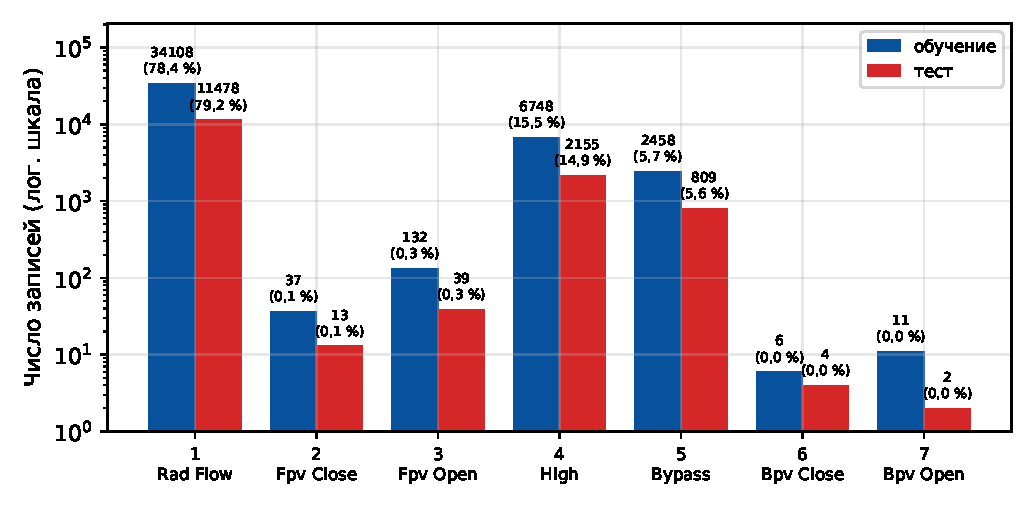
\includegraphics[width=0.95\textwidth]{figures/fig1_classes.pdf}
\caption{Распределение классов в обучающей и тестовой частях
(логарифмическая шкала)}
\label{fig:classes}
\end{figure}

Пропусков нет, полных дубликатов нет, пересечение обучающей и тестовой
частей равно \NOverlap. Все \NFeatures{} признаков принимают
содержательные значения и различаются по масштабу: одни укладываются
в десятки, другие~--- в тысячи. Для линейных моделей, kNN и SVM это
означает необходимость стандартизации; деревья и их ансамбли
к масштабу нечувствительны, что отдельно проверено в
разделе~\ref{sec:scaling}.

Дисбаланс классов хорошо виден на рисунке~\ref{fig:classes}: класс 1
доминирует, классы 4 и 5 образуют второй эшелон, а классы 2, 3, 6 и 7
представлены единицами или десятками записей. В тестовой части класс 7
встречается \SupportClassSeven{} раза, класс 6~--- \SupportClassSix{}
раза. Этого достаточно, чтобы оценить работу модели качественно, но
недостаточно для устойчивой количественной оценки: одна ошибка меняет
F1 такого класса в разы.

\subsection{Исследовательские вопросы}

До обучения сформулированы три гипотезы.

\begin{description}
  \item[H1 (разделимость).] Редкие классы отделимы от остальных по
  нескольким признакам: крайние значения B характерны для классов 6 и 7,
  а комбинации A, C, H и I помогают различить классы 2 и 3. Если это так,
  деревья и ансамбли должны работать почти идеально, а ошибки будут
  единичными.
  \item[H2 (ловушка accuracy).] Высокая accuracy совместима с низким
  macro-F1: модель может почти не ошибаться на доминирующем классе
  и при этом терять редкие классы. Величина разрыва зависит от того,
  насколько равномерно модель «размазывает» ошибки по классам.
  \item[H3 (устойчивость ансамблей).] Случайный лес и градиентный бустинг
  устойчивее одиночного дерева и линейных моделей на редких классах,
  потому что усредняют много деревьев и лучше используют локальную
  структуру признакового пространства.
\end{description}

Исследовательский вопрос работы: какие именно редкие классы смешиваются,
с какими классами и почему при accuracy выше 99~\% macro-F1 может быть
существенно ниже.

% ============================================================================
\section{МЕТОДИКА}

\subsection{Признаки и предобработка}
\label{sec:scaling}

Используются все \NFeatures{} числовых признаков A--I без ручного
конструирования. Никаких преобразований, зависящих от целевой переменной,
не выполняется. Для логистической регрессии, kNN и SVM стандартизация
включена в конвейер \texttt{Pipeline} и обучается только на обучающих
складках, поэтому информация из проверочной части не просачивается
в масштаб.

Для деревьев, случайного леса и бустинга масштабирование не требуется:
разбиение узла зависит от порядка значений, а не от расстояний. Это
проверено отдельно: одна и та же настроенная модель обучалась с
\texttt{StandardScaler} и без него в пятикратной кросс-валидации.
Результаты совпали: дерево~--- \ScaleTreeRaw{} и \ScaleTreeScaled,
случайный лес~--- \ScaleRfRaw{} и \ScaleRfScaled, бустинг~---
\ScaleHgbRaw{} и \ScaleHgbScaled. Совпадение ожидаемо, но полезно как
проверка отсутствия скрытых зависимостей от масштаба.

\subsection{Разбиение и кросс-валидация}

Внешнее разбиение задано авторами набора и не меняется: \NTrain{} записей
обучения и \NTest{} теста. Тестовая часть открывается один раз, после
выбора окончательной модели. Все решения~--- выбор гиперпараметров,
сравнение моделей, проверка масштабирования~--- принимаются только
по обучающей части.

Внутри обучения используется стратифицированная пятикратная
кросс-валидация \texttt{StratifiedKFold} с перемешиванием и фиксированным
\texttt{random\_state}=42. Стратификация важна: без неё редкие классы
могли бы вообще не попасть в отдельные складки, и оценка стала бы
случайной. Для методических экспериментов с деревьями и ансамблями
дополнительно выделяется 20~\% обучающей части как проверочная; это
внутренняя проверка, а не тест авторов набора.

\subsection{Модели}

Сравниваются семь моделей, покрывающих основные семейства алгоритмов.

\begin{enumerate}
  \item \textbf{Dummy} (\texttt{most\_frequent})~--- базовая модель,
  всегда предсказывающая класс 1. Она показывает, какую accuracy даёт
  полное игнорирование задачи.
  \item \textbf{Логистическая регрессия} со стандартизацией, подбором
  коэффициента $C$ и весов классов. Линейная модель служит эталоном
  «простого» решения и позволяет интерпретировать коэффициенты.
  \item \textbf{kNN} со стандартизацией, подбором числа соседей и веса
  голосов. Метод не строит явной границы и чувствителен к локальной
  плотности классов.
  \item \textbf{SVM с RBF-ядром} со стандартизацией, подбором $C$,
  $\gamma$ и весов классов. Ядровая машина хорошо работает на компактных
  классах и даёт непрерывные оценки для ROC-анализа.
  \item \textbf{Решающее дерево} с ограничением глубины и минимального
  листа. Дерево интерпретируемо и служит основой для ансамблей.
  \item \textbf{Случайный лес}~--- бэггинг деревьев с случайным
  подмножеством признаков. Он снижает разброс одиночного дерева.
  \item \textbf{HistGradientBoosting}~--- современный градиентный
  бустинг, встроенный в scikit-learn~\cite{sklearn}. Выбран потому, что
  не требует внешних зависимостей, поддерживает многоклассовую задачу,
  веса классов и быстро обучается на табличных данных.
\end{enumerate}

Все модели реализованы средствами scikit-learn~\cite{sklearn}; случайные
состояния зафиксированы. Для ансамблей и бустинга это особенно важно:
без фиксации \texttt{random\_state} разброс между запусками мог бы
превысить различия между моделями.

\subsection{Подбор гиперпараметров}

Подбор выполняется двумя способами. Для моделей с небольшим числом
параметров используется \texttt{GridSearchCV}, для бустинга~---
\texttt{RandomizedSearchCV} с 24 конфигурациями. Оба поиска оптимизируют
macro-F1 на пяти складках обучающей части.

Сетки и выбранные значения приведены в таблице~\ref{tab:search}.
Логистическая регрессия перебирает $C$ и вариант весов классов; kNN~---
число соседей и способ взвешивания; SVM~--- $C$, $\gamma$ и веса классов;
дерево~--- глубину и минимальный лист; лес~--- глубину, минимальный лист
и долю признаков; бустинг~--- скорость обучения, число итераций, число
листьев, минимальный лист, $l_2$-регуляризацию и веса классов.

\begin{table}[H]
\centering
\small
\caption{Основные гиперпараметры окончательной модели}
\label{tab:bestparams}
\begin{tabular}{ll}
\toprule
Параметр & Значение \\
\midrule
Модель & \BestName \\
Веса классов & \HgbClassWeight \\
Скорость обучения & \HgbBestLr \\
Число итераций & \HgbBestIter \\
Максимум листьев & \HgbBestLeaf \\
$l_2$-регуляризация & \HgbBestLTwo \\
\bottomrule
\end{tabular}
\end{table}

\subsection{Метрики и статистическая надёжность}

Вычисляются accuracy, сбалансированная accuracy, macro-F1, weighted-F1
и ROC-AUC one-vs-rest по непрерывным оценкам. Основная метрика~---
macro-F1:
\begin{equation}
\mathrm{macro\text{-}F1} = \frac{1}{K}\sum_{k=1}^{K} F1_k,
\label{eq:macrof1}
\end{equation}
где $K=\NClasses$~--- число классов, а $F1_k$ считается по схеме
«один против всех». В отличие от accuracy, каждый класс входит в сумму
с одинаковым весом, поэтому провал на редком классе не растворяется
в потоке правильных ответов на классе 1.

Accuracy полезна как прикладная характеристика: она отвечает на вопрос
«какую долю записей модель классифицирует верно». Но при дисбалансе
она не различает «модель выучила все классы» и «модель выучила только
самый частый». Сбалансированная accuracy усредняет recall по классам
и частично закрывает этот пробел, однако не учитывает precision.
Поэтому в работе приводятся все перечисленные метрики, а решение
принимается по macro-F1.

ROC-AUC считается как среднее бинарных AUC «один против всех» по
непрерывным оценкам модели. Для моделей с \texttt{predict\_proba}
используются вероятности, для SVM~--- значения решающей функции.
Макро-AUC показывает, насколько хорошо модель упорядочивает объекты
каждого класса, но при почти идеальной разделимости быстро насыщается
единицей и перестаёт различать модели.

Отдельно оговаривается статистическая надёжность. В тестовой части
класс 2 представлен \SupportClassTwo{} примерами, класс 3~---
\SupportClassThree, класс 6~--- \SupportClassSix, класс 7~---
\SupportClassSeven. Для классов 6 и 7 доверительные интервалы метрик
практически совпадают с отрезком от нуля до единицы: одна ошибка
переводит F1 из единицы в половину или две трети. Поэтому выводы
по этим классам носят иллюстративный характер, а не характер
устойчивой количественной оценки.

% ============================================================================
\section{РЕЗУЛЬТАТЫ}

\subsection{Разведочный анализ}

На рисунке~\ref{fig:domain} показаны обучающие объекты в координатах
двух пар признаков. Левая панель (A--C) показывает, что класс 1 образует
плотное облако, классы 4 и 5 примыкают к нему, а классы 2, 3, 6 и 7
образуют отдельные компактные группы. Правая панель (A--B,
симметричная логарифмическая шкала) делает наглядными крайние значения
признака B: классы 6 и 7 расположены далеко вверх и вниз, тогда как
основная масса классов 1, 4 и 5 сосредоточена около нуля.

\begin{figure}[H]
\centering
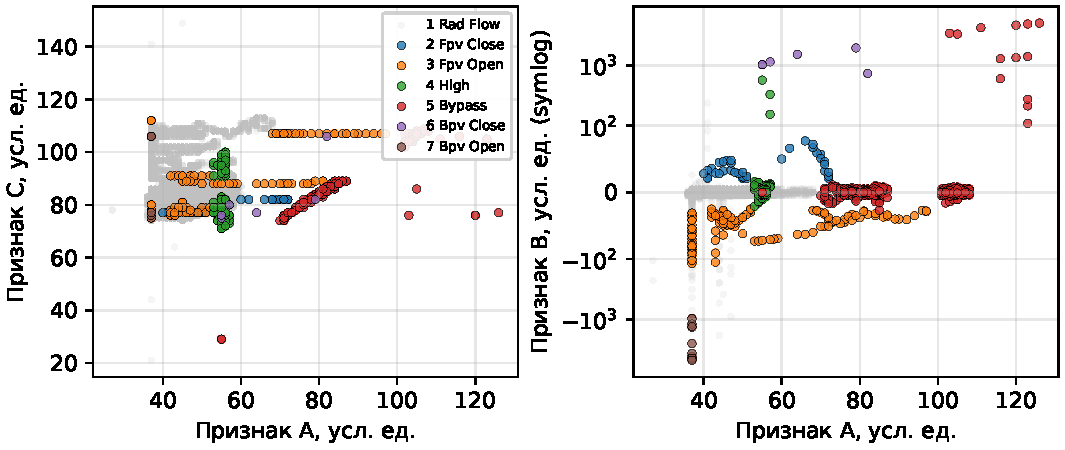
\includegraphics[width=\textwidth]{figures/fig2_domain.pdf}
\caption{Обучающие объекты в координатах A--C (слева) и A--B
(справа, симметричная логарифмическая шкала)}
\label{fig:domain}
\end{figure}

Уже на этом этапе видны две вещи. Во-первых, редкие классы не
разбросаны по всему пространству, а занимают характерные области:
это объясняет, почему деревья и ансамбли работают почти идеально.
Во-вторых, классы 2 и 4 частично перекрываются по A и C, а различаются
другими признаками; именно здесь возникает единственная содержательная
ошибка окончательной модели. Гипотеза H1 в целом подтверждается:
редкие классы отделимы, но не по одной паре координат, а по совокупности
\NFeatures{} показаний.

\subsection{Сравнение моделей}

Результаты кросс-валидации и однократной проверки на тесте собраны
в таблице~\ref{tab:models} и на рисунке~\ref{fig:models}. Матрицы ошибок
всех моделей показаны на рисунке~\ref{fig:confusionall}.

\begin{table}[H]
\centering
\footnotesize
\caption{Качество моделей: кросс-валидация на обучении и однократная проверка на тесте}\label{tab:models}
\resizebox{\textwidth}{!}{%
\begin{tabular}{lcccccc}
\toprule
Модель & CV macro-F1 & Тест, accuracy & Bal. accuracy & Macro-F1 & Weighted-F1 & ROC-AUC \\
\midrule
Dummy (most frequent) & 0,13 $\pm$ 0,00 & 0,7916 & 0,14 & 0,13 & 0,70 & 0,50 \\
Логистическая регрессия & 0,86 $\pm$ 0,05 & 0,9539 & 0,99 & 0,82 & 0,96 & 1,00 \\
kNN & 0,93 $\pm$ 0,02 & 0,9991 & 0,87 & 0,88 & 1,00 & 0,93 \\
SVM (RBF) & 0,91 $\pm$ 0,02 & 0,9976 & 0,91 & 0,84 & 1,00 & 1,00 \\
Решающее дерево & 0,95 $\pm$ 0,07 & 0,9999 & 0,99 & 0,99 & 1,00 & 0,99 \\
Случайный лес & 0,94 $\pm$ 0,08 & 0,9999 & 0,99 & 0,99 & 1,00 & 1,00 \\
Градиентный бустинг (HistGB) & 0,96 $\pm$ 0,06 & 0,9999 & 0,99 & 0,99 & 1,00 & 1,00 \\
\bottomrule
\end{tabular}}
\end{table}

\begin{figure}[H]
\centering
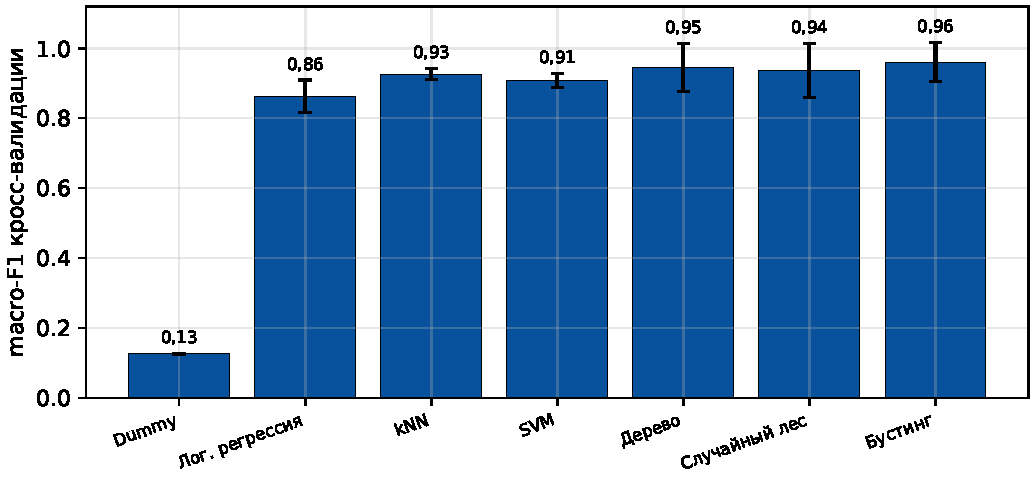
\includegraphics[width=0.95\textwidth]{figures/fig3_models.pdf}
\caption{Macro-F1 кросс-валидации для всех моделей (усы~--- стандартное
отклонение по складкам)}
\label{fig:models}
\end{figure}

\begin{figure}[H]
\centering
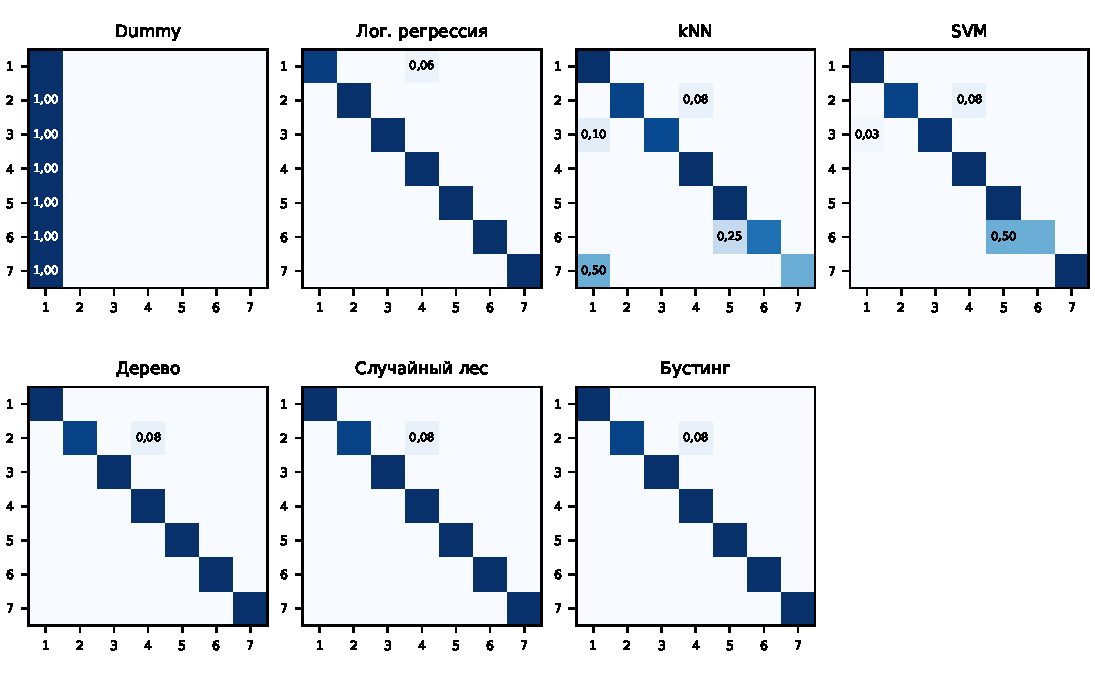
\includegraphics[width=\textwidth]{figures/fig13_confusion_all.pdf}
\caption{Нормированные матрицы ошибок всех моделей на тесте; подписаны
только ненулевые внедиагональные элементы}
\label{fig:confusionall}
\end{figure}

Базовая модель даёт accuracy \AccDummy{} и macro-F1 \FOneDummy: это
точка отсчёта, ниже которой не должна опускаться ни одна содержательная
модель. Логистическая регрессия резко улучшает macro-F1 до \FOneLogreg,
но проигрывает по accuracy (\AccLogreg): сбалансированные веса заставляют
её активно предсказывать редкие классы, что повышает recall, но снижает
precision. kNN и SVM, наоборот, дают очень высокую accuracy
(\AccKnn{} и \AccSvm) при macro-F1 \FOneKnn{} и \FOneSvm. Дерево, лес
и бустинг выходят на почти идеальный уровень: accuracy \AccTree,
\AccRf, \AccHgb, macro-F1 \FOneTree, \FOneRf, \FOneHgb.

По правилу выбора «лучшая macro-F1 кросс-валидации» побеждает
«\BestName» с результатом $\BestCvF \pm \BestCvFStd$. Обратим внимание:
на тесте у дерева и леса macro-F1 чуть выше, чем у бустинга
(\FOneTree{} и \FOneRf{} против \FOneHgb). Разница меньше одной ошибки
на \NTest{} объектов и находится в пределах статистического шума.
Именно поэтому модель выбирается по кросс-валидации, а не по тесту:
выбор по тесту был бы подгонкой под ответ.

\subsection{Подбор гиперпараметров}

Выбранные параметры и пространства поиска приведены в
таблице~\ref{tab:search}, визуализация поиска~--- на
рисунке~\ref{fig:search}.

\begin{table}[H]
\centering
\footnotesize
\setlength{\tabcolsep}{3pt}
\caption{Подбор гиперпараметров: поиск, выбранные значения и оценка кросс-валидации}\label{tab:search}
\begin{tabular}{@{}>{\raggedright\arraybackslash}p{2.4cm}>{\raggedright\arraybackslash}p{1.5cm}>{\raggedright\arraybackslash}p{4.1cm}>{\raggedright\arraybackslash}p{4.2cm}r@{}}
\toprule
Модель & Поиск & Пространство & Лучшие параметры & CV macro-F1 \\
\midrule
Dummy (most frequent) & --- & --- & --- & 0,13 \\
Логистическая регрессия & Grid, $5\times2$ & $C\in\{0{,}01;\ldots;100\}$; class\_weight & C=1, class\_weight=balanced & 0,86 \\
kNN & Grid, $5\times2$ & $k\in\{1;3;5;9;15\}$; weights & n\_neighbors=1, weights=uniform & 0,93 \\
SVM (RBF) & Grid, $3\times2\times2$ & $C\in\{1;10;100\}$; $\gamma\in\{0{,}01;0{,}1\}$; class\_weight & C=100, class\_weight=balanced, gamma=0,01 & 0,91 \\
Решающее дерево & Grid, $7\times4$ & max\_depth; min\_samples\_leaf & max\_depth=10, min\_samples\_leaf=1 & 0,95 \\
Случайный лес & Grid, $1\times3\times2\times2$ & max\_depth; min\_samples\_leaf; max\_features & max\_depth=10, max\_features=0,5, min\_samples\_leaf=1, n\_estimators=200 & 0,94 \\
Градиентный бустинг (HistGB) & Random, 24 & learning\_rate; max\_iter; max\_leaf\_nodes; min\_samples\_leaf; $l_2$ & class\_weight=balanced, l2\_regularization=0, learning\_rate=0,056, max\_iter=100, max\_leaf\_nodes=31, min\_samples\_leaf=10 & 0,96 \\
\bottomrule
\end{tabular}
\end{table}

\begin{figure}[H]
\centering
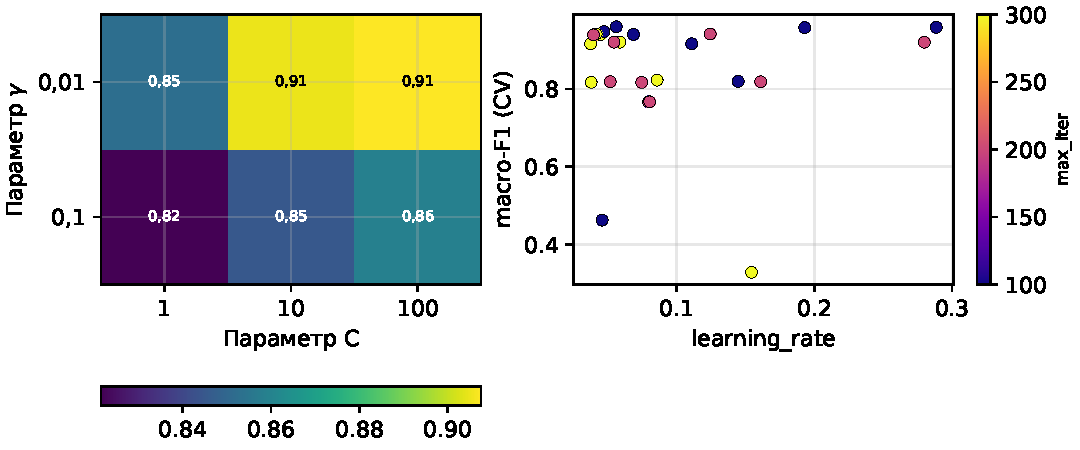
\includegraphics[width=\textwidth]{figures/fig8_search.pdf}
\caption{Подбор гиперпараметров: macro-F1 для SVM по $C$ и $\gamma$
(слева) и облако конфигураций бустинга (справа)}
\label{fig:search}
\end{figure}

Для SVM лучшей оказалась комбинация $C=\SvcBestC$, $\gamma=\SvcBestGamma$
с весами классов; CV macro-F1 равна \SvcSearchF. На левой панели видно,
что малое $\gamma$ устойчиво лучше большого: при $\gamma=0{,}01$ все
значения $C$ дают результат выше, чем при $\gamma=0{,}1$. Слишком
гибкое ядро подстраивается под доминирующий класс и теряет редкие.

Для бустинга случайный поиск выбрал скорость обучения \HgbBestLr,
\HgbBestIter{} итераций, \HgbBestLeaf{} листьев, минимальный лист
и $l_2$-регуляризацию \HgbBestLTwo{} с весами классов
«\HgbClassWeight»; CV macro-F1 равна \HgbSearchF. На правой панели
заметна одна конфигурация с macro-F1 около 0{,}3~--- это пример
неудачного сочетания большой скорости обучения и числа итераций,
при котором модель на промежуточных шагах теряет редкие классы.
Поиск её отбросил.

\subsection{Переобучение решающего дерева}

Одиночное дерево~--- самый наглядный пример переобучения. На
рисунке~\ref{fig:tree} показаны зависимости ошибки и логарифмической
потери от глубины и минимального размера листа.

\begin{figure}[H]
\centering
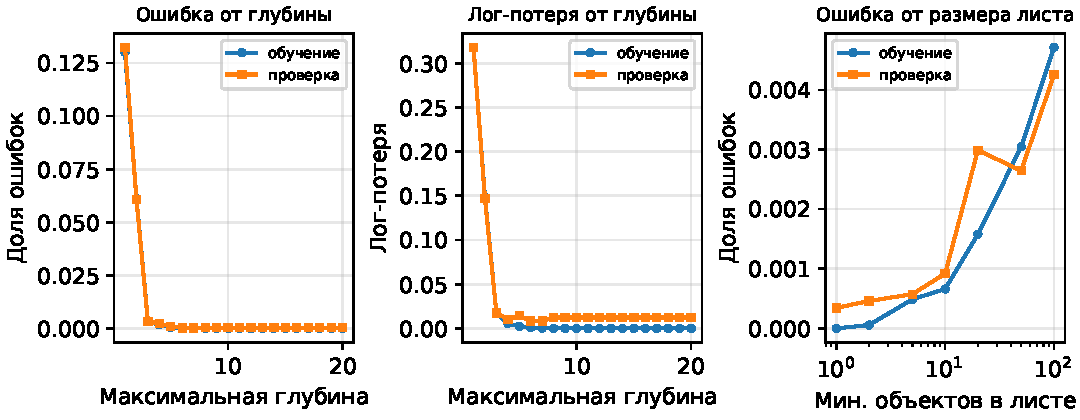
\includegraphics[width=\textwidth]{figures/fig4_tree_overfit.pdf}
\caption{Решающее дерево: ошибка от глубины (слева), лог-потеря
от глубины (в центре), ошибка от минимального размера листа (справа)}
\label{fig:tree}
\end{figure}

Доля ошибок на обучении падает почти до нуля уже при глубине
\TreeBestDepth, и по ней трудно заметить переобучение: на проверке
ошибка тоже близка к нулю (\TreeBestValErr). Логарифмическая потеря
чувствительнее. При глубине \TreeBestDepth{} она минимальна
(\TreeBestValLl), а при дальнейшем росте глубины обучение уходит
в ноль (\TreeDeepTrainLl), тогда как проверка ухудшается до
\TreeDeepValLl. Это классическая картина: дерево запоминает обучающие
объекты и становится переуверенным, хотя доля ошибок почти не меняется.
Именно поэтому в экспериментах с деревьями и лесами мы смотрим и на
ошибку, и на лог-потерю.

Минимальный размер листа работает как регуляризатор: лучшее значение
на проверке~--- \TreeBestLeaf, при увеличении листа ошибка растёт.
Отметим, что поиск по кросс-валидации выбрал для итогового дерева
глубину из таблицы~\ref{tab:search}, а не \TreeBestDepth: различия
между глубинами в этом диапазоне лежат в пределах разброса складок,
а кросс-валидация использует всю обучающую часть, а не одно разбиение.

\subsection{Случайный лес: число деревьев и параметры}

Зависимость качества леса от числа деревьев показана на
рисунке~\ref{fig:rfntrees}. С ростом числа деревьев ошибка падает
с \RfTreeErr{} у одного дерева до \RfErrFinal{} при \RfNfinal{} деревьях,
а лог-потеря~--- с \RfTreeLl{} до \RfLlFinal. Разброс по трём значениям
\texttt{random\_state} быстро уменьшается: уже при ста деревьях
стандартное отклонение лог-потери равно \RfLlStdFinal. Это иллюстрирует
главное свойство бэггинга: усреднение независимых деревьев снижает
дисперсию, а не смещение.

\begin{figure}[H]
\centering
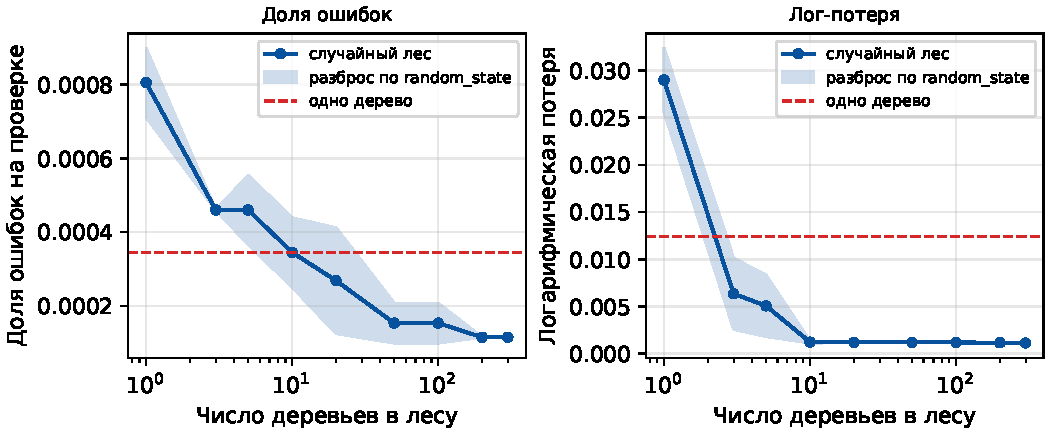
\includegraphics[width=\textwidth]{figures/fig5_rf_ntrees.pdf}
\caption{Случайный лес: доля ошибок (слева) и лог-потеря (справа)
в зависимости от числа деревьев; пунктир~--- одно дерево}
\label{fig:rfntrees}
\end{figure}

Влияние трёх гиперпараметров леса показано в верхнем ряду
рисунка~\ref{fig:params}. По доле ошибок глубина 10 и больше
неразличима (\RfExpErrDepth), поэтому для выбора приходится смотреть
на лог-потеря: она минимальна при глубине \RfExpLlBestDepth{}
(\RfExpLlDepth). Минимальный лист \RfExpBestLeaf{} даёт лучший результат,
а увеличение листа монотонно ухудшает лог-потерю. Доля признаков
в разбиении~--- самый тонкий параметр: по ошибке оптимум приходится на
\RfExpBestFeat, по лог-потере~--- на \RfExpLlBestFeat, причём разница
между значениями мала (\RfExpLlFeat). Поиск по macro-F1 выбрал
компромиссное значение из таблицы~\ref{tab:search}. Этот пример хорошо
показывает, что при почти нулевой ошибке разные метрики могут указывать
на разные оптимумы.

\subsection{Градиентный бустинг: кривые и параметры}

Кривые бустинга при двух скоростях обучения показаны на
рисунке~\ref{fig:gbiters}. Левая панель~--- доля ошибок, правая~---
логарифмическая потеря. Доля ошибок быстро выходит на плато
\GbErrLowFinal{} и дальше не меняется: по ней переобучение незаметно.
Лог-потеря ведёт себя иначе. При скорости \GbLrHigh{} минимум
\GbLlMinHigh{} достигается на \GbLlIterHigh{} итерации, при скорости
\GbLrLow{} минимум \GbLlMinLow{}~--- на \GbLlIterLow. После минимума
лог-потеря растёт до \GbLlFinalLow{} и \GbLlFinalHigh{}: модель
становится переуверенной, хотя продолжает классифицировать те же объекты
правильно.

\begin{figure}[H]
\centering
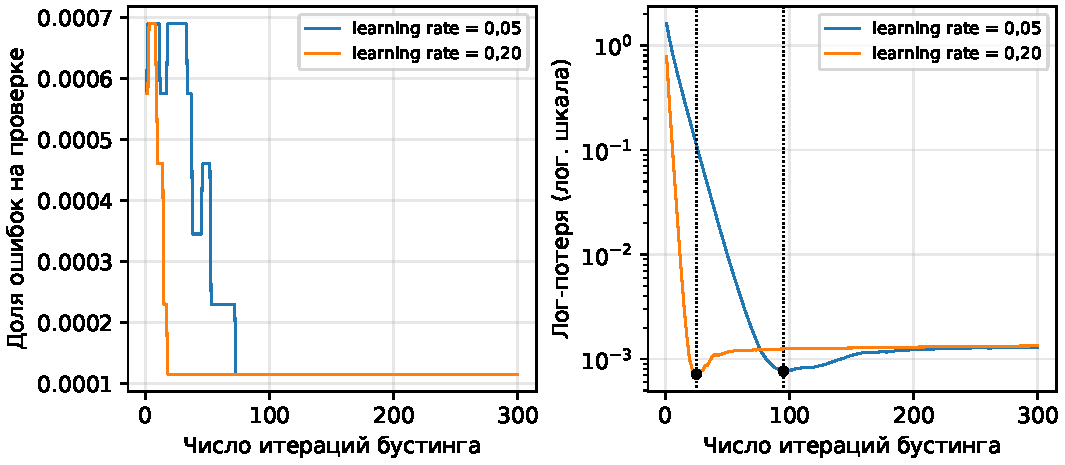
\includegraphics[width=\textwidth]{figures/fig6_gb_iters.pdf}
\caption{Градиентный бустинг при двух скоростях обучения: доля ошибок
(слева) и лог-потеря (справа); точками отмечены минимумы}
\label{fig:gbiters}
\end{figure}

Соотношение скоростей соответствует теории~\cite{friedman}: меньший шаг
требует больше итераций до оптимума, но и позже начинает переобучаться.
Именно поэтому в окончательной модели используются и веса классов,
и ограниченное число итераций: без балансировки весов промежуточные
итерации на сильно несбалансированных данных становятся неустойчивыми.

Влияние трёх гиперпараметров бустинга показано в нижнем ряду
рисунка~\ref{fig:params}. Слишком большая скорость обучения резко
ухудшает результат, оптимальная по проверке~--- \GbExpBestLr{}
(\GbExpErrLr). Число итераций \GbExpBestIter{} даёт ошибку
\GbExpErrIter, а число листьев \GbExpBestLeaf{}~--- \GbExpErrLeaf.
Поиск по кросс-валидации выбрал близкие, но не совпадающие значения
(таблица~\ref{tab:search}): совместная оптимизация шести параметров
и пяти складок допускает несколько почти эквивалентных конфигураций.

\begin{figure}[H]
\centering
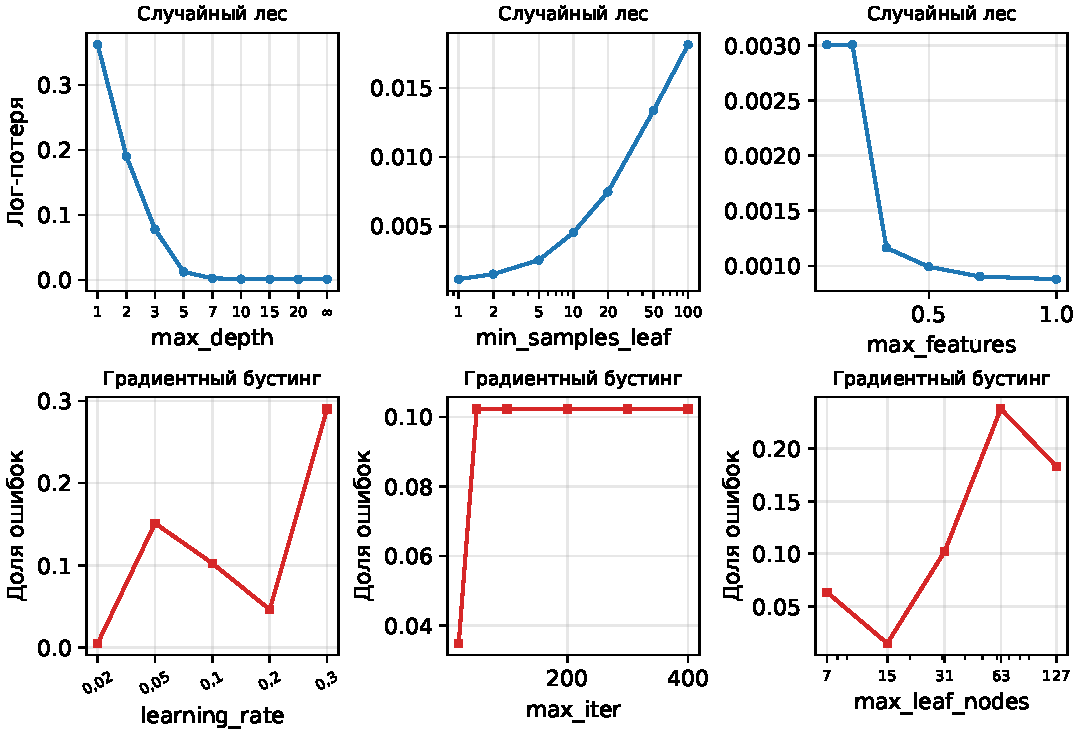
\includegraphics[width=\textwidth]{figures/fig7_rf_gb_params.pdf}
\caption{Влияние гиперпараметров: случайный лес по лог-потере (верхний
ряд) и градиентный бустинг по доле ошибок (нижний ряд)}
\label{fig:params}
\end{figure}

\subsection{Окончательная модель и матрица ошибок}

Окончательная модель~--- «\BestName» с параметрами
\BestParams. Её метрики на тесте: accuracy \BestAcc, сбалансированная
accuracy \BestBal, macro-F1 \BestFOne, weighted-F1 \BestWf,
macro-ROC-AUC \BestAuc. Нормированная матрица ошибок показана на
рисунке~\ref{fig:confusion}, метрики по классам~--- в
таблице~\ref{tab:class} и на рисунке~\ref{fig:perclass}.

\begin{figure}[H]
\centering
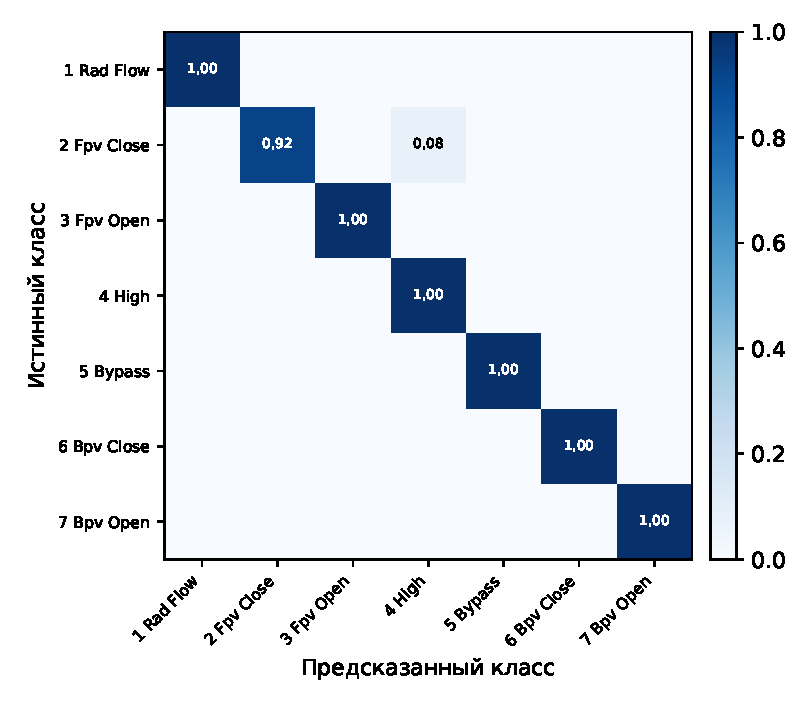
\includegraphics[width=0.72\textwidth]{figures/fig9_confusion.pdf}
\caption{Нормированная матрица ошибок окончательной модели на тесте}
\label{fig:confusion}
\end{figure}

\begin{table}[H]
\centering
\small
\caption{Метрики окончательной модели по классам (тест)}\label{tab:class}
\begin{tabular}{clrrrr}
\toprule
Класс & Состояние & Precision & Recall & F1 & Поддержка \\
\midrule
1 & Rad Flow & 1,00 & 1,00 & 1,00 & 11478 \\
2 & Fpv Close & 1,00 & 0,92 & 0,96 & 13 \\
3 & Fpv Open & 1,00 & 1,00 & 1,00 & 39 \\
4 & High & 1,00 & 1,00 & 1,00 & 2155 \\
5 & Bypass & 1,00 & 1,00 & 1,00 & 809 \\
6 & Bpv Close & 1,00 & 1,00 & 1,00 & 4 \\
7 & Bpv Open & 1,00 & 1,00 & 1,00 & 2 \\
\bottomrule
\end{tabular}
\end{table}

\begin{figure}[H]
\centering
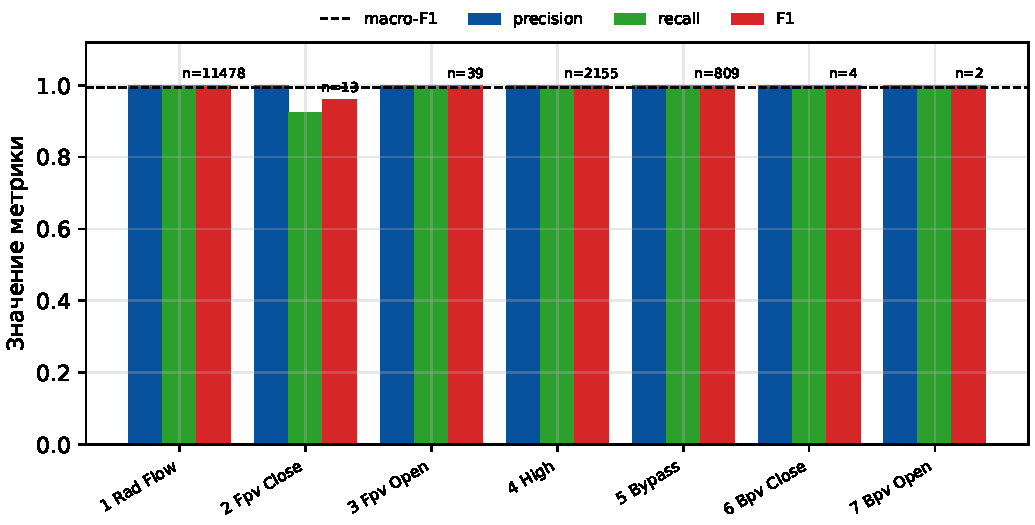
\includegraphics[width=0.95\textwidth]{figures/fig10_per_class.pdf}
\caption{Precision, recall и F1 окончательной модели по классам;
$n$~--- число тестовых примеров}
\label{fig:perclass}
\end{figure}

Матрица почти диагональна. Единственная содержательная ошибка~---
\ConfCntTwoFour{} объект класса 2, отнесённый к классу 4: это одна запись
из \SupportClassTwo. Вторая ошибка~--- объект класса 1, предсказанный
как класс 5; в нормированной матрице она округляется до нуля, потому что
класс 1 содержит \SupportClassOne{} объектов. Все остальные классы,
включая редкие 3, 6 и 7, распознаны полностью.

По классам F1 равен \FOneClassOne, \FOneClassTwo, \FOneClassThree,
\FOneClassFour, \FOneClassFive, \FOneClassSix, \FOneClassSeven. Класс 2
единственный имеет F1 ниже единицы (\FOneClassTwo) из-за recall
\RecClassTwo: одна пропущенная запись на \SupportClassTwo{} даёт такую
просадку. Для классов 6 и 7 значения \FOneClassSix{} и \FOneClassSeven{}
выглядят идеально, но опираются на \SupportClassSix{} и
\SupportClassSeven{} примеров; доверять этим числам как устойчивой
оценке нельзя.

\subsection{ROC-анализ}

ROC-кривые окончательной модели показаны на рисунке~\ref{fig:roc},
AUC по классам для трёх моделей~--- в таблице~\ref{tab:auc}.

\begin{figure}[H]
\centering
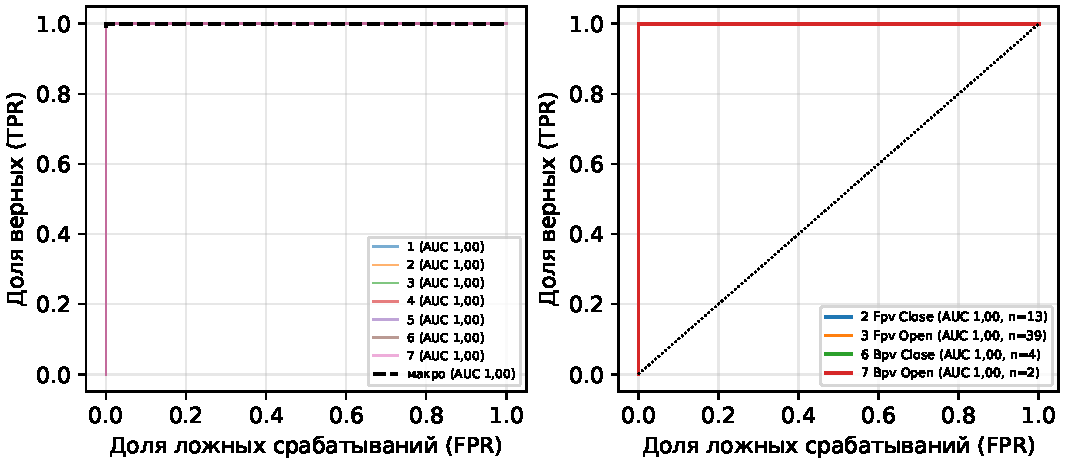
\includegraphics[width=\textwidth]{figures/fig11_roc.pdf}
\caption{ROC-кривые окончательной модели: все классы и макро-усреднение
(слева), редкие классы 2, 3, 6 и 7 (справа)}
\label{fig:roc}
\end{figure}

\begin{table}[H]
\centering
\small
\caption{AUC one-vs-rest по классам на тесте}\label{tab:auc}
\begin{tabular}{clccc}
\toprule
Класс & Состояние & Окончательная & Лог. регрессия & Случайный лес \\
\midrule
1 & Rad Flow & 1,00 & 0,99 & 1,00 \\
2 & Fpv Close & 1,00 & 1,00 & 1,00 \\
3 & Fpv Open & 1,00 & 1,00 & 1,00 \\
4 & High & 1,00 & 0,99 & 1,00 \\
5 & Bypass & 1,00 & 1,00 & 1,00 \\
6 & Bpv Close & 1,00 & 1,00 & 1,00 \\
7 & Bpv Open & 1,00 & 1,00 & 1,00 \\
\midrule
 & Macro & 1,00 & 1,00 & 1,00 \\
\bottomrule
\end{tabular}
\end{table}

У окончательной модели AUC всех классов равен \AucClassOne{} с точностью
до двух знаков: данные почти разделимы, и ROC-кривые прижимаются к
левому верхнему углу. Macro-AUC \BestAuc{} не различает модели: у
случайного леса он тоже \AucRf, а у логистической регрессии~--- \AucLogreg.
Различие проявляется не в упорядочивании, а в единичных решениях при
выборе порога. Поэтому ROC-AUC в этой задаче полезен как проверка
качества ранжирования, но не как критерий выбора модели. Основную
информацию несёт macro-F1, чувствительный к редким классам.

\subsection{Интерпретация признаков}

Важность признаков окончательной модели, измеренная перестановкой на
отложенной части обучения, показана на рисунке~\ref{fig:importance}
и в таблице~\ref{tab:importance}. Рядом приведены коэффициенты
логистической регрессии~--- они дают альтернативный, линейный взгляд
на те же данные.

\begin{figure}[H]
\centering
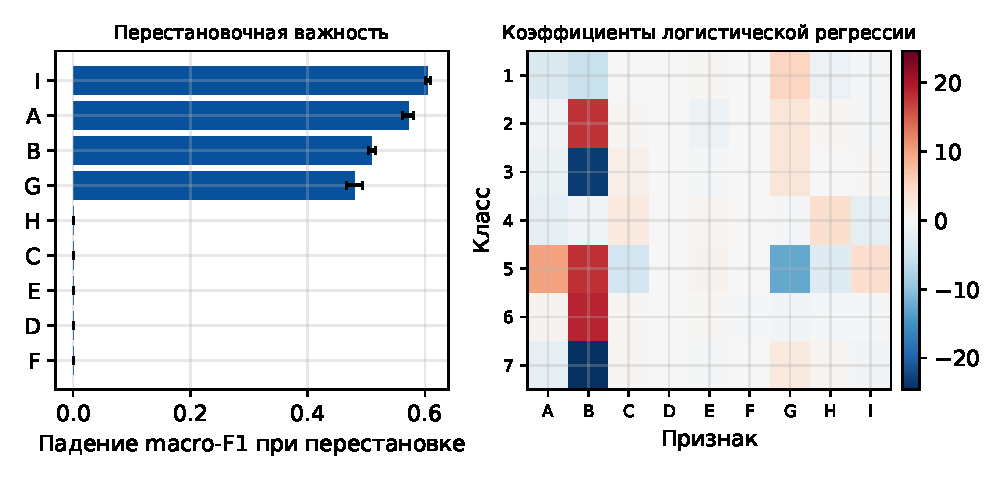
\includegraphics[width=\textwidth]{figures/fig12_importance.pdf}
\caption{Перестановочная важность окончательной модели (слева)
и коэффициенты логистической регрессии по классам (справа)}
\label{fig:importance}
\end{figure}

Наибольший вклад вносит признак \ImpTopFeature{} (\ImpTopValue{}),
за ним следует \ImpSecondFeature{} (\ImpSecondValue). Признаки C, D, E
и F почти не влияют на macro-F1: их перестановка не меняет метрику
сколько-нибудь заметно. Коэффициенты логистической регрессии показывают,
что классы 2, 3 и 7 опираются в первую очередь на признак B, а класс 5~
--- на комбинацию A и G. Поскольку физический смысл признаков не раскрыт,
мы не можем сказать, какие именно датчики стоят за этими номерами;
интерпретация остаётся статистической, а не физической. Это ограничение
честно зафиксировано в постановке задачи.

\begin{table}[H]
\centering
\small
\caption{Перестановочная важность признаков окончательной модели (падение macro-F1)}\label{tab:importance}
\begin{tabular}{clrr}
\toprule
Место & Признак & Среднее падение & Стандартное отклонение \\
\midrule
1 & I & 0,60 & 0,00 \\
2 & A & 0,57 & 0,01 \\
3 & B & 0,51 & 0,01 \\
4 & G & 0,48 & 0,01 \\
5 & H & 0,00 & 0,00 \\
6 & C & 0,00 & 0,00 \\
7 & E & 0,00 & 0,00 \\
8 & D & 0,00 & 0,00 \\
9 & F & 0,00 & 0,00 \\
\bottomrule
\end{tabular}
\end{table}

% ============================================================================
\section{ОБСУЖДЕНИЕ: РЕДКИЕ КЛАССЫ И ЛОВУШКА ACCURACY}

\subsection{Какие классы смешиваются}

Главная ошибка окончательной модели~--- класс 2, предсказанный как
класс 4. Классы 2 (Fpv Close) и 4 (High) действительно близки по
нескольким признакам и различаются совокупностью показаний, а не одной
координатой. На тесте класса 2 всего \SupportClassTwo{} объектов,
поэтому одна ошибка даёт recall \RecClassTwo{} и F1 \FOneClassTwo.
У дерева, леса и бустинга это единственная повторяющаяся ошибка
(рисунок~\ref{fig:confusionall}).

Вторая группа смешения~--- классы 3 и 1. У SVM
\ConfCntSvmThreeOne{} из \SupportClassThree{} объектов класса 3
(доля \ConfSvmThreeOne) уходит в класс 1, а \ConfCntSvmOneThree{} объектов
класса 1~--- в класс 3. Это уже не единичная ошибка, а систематическая
путаница на границе: класс 3 (Fpv Open) по части признаков похож на
доминирующий класс 1. В результате precision класса 3 падает до
\PrecSvmClassThree, хотя accuracy модели остаётся \AccSvm. Именно такие
ошибки accuracy не видит: \ConfCntSvmOneThree{} от \SupportClassOne{}
объектов~--- это доли процента, но для класса из
\SupportClassThree{} примеров они критичны.

Третья группа~--- классы 6 и 7. Они хорошо отделены по признаку B,
но их тестовые представительства равны \SupportClassSix{} и
\SupportClassSeven. У kNN класс 7 распознан с F1 \FOneKnnClassSeven:
одна ошибка на два объекта. У SVM F1 классов 6 и 7 равны
\FOneSvmClassSix{} и \FOneSvmClassSeven. Эти числа выглядят тревожно,
но их доверительные интервалы огромны: сдвиг одного объекта меняет
метрику на десятки процентов.

Сводка F1 по всем классам и всем моделям приведена в
таблице~\ref{tab:classmodels}. Она показывает, что разрыв между
моделями возникает почти исключительно на редких классах 2, 3, 6 и 7:
по классам 1, 4 и 5 все содержательные модели практически неразличимы.

\begin{table}[H]
\centering
\footnotesize
\caption{F1 по классам на тесте для всех моделей}\label{tab:classmodels}
\resizebox{\textwidth}{!}{%
\begin{tabular}{clrrrrrr}
\toprule
Класс & Состояние & Лог. регр. & kNN & SVM & Дерево & Лес & Бустинг \\
\midrule
1 & Rad Flow & 0,97 & 1,00 & 1,00 & 1,00 & 1,00 & 1,00 \\
2 & Fpv Close & 0,76 & 0,96 & 0,83 & 0,96 & 0,96 & 0,96 \\
3 & Fpv Open & 0,85 & 0,92 & 0,75 & 0,99 & 1,00 & 1,00 \\
4 & High & 0,87 & 1,00 & 1,00 & 1,00 & 1,00 & 1,00 \\
5 & Bypass & 1,00 & 1,00 & 1,00 & 1,00 & 1,00 & 1,00 \\
6 & Bpv Close & 0,73 & 0,86 & 0,67 & 1,00 & 1,00 & 1,00 \\
7 & Bpv Open & 0,57 & 0,40 & 0,67 & 1,00 & 1,00 & 1,00 \\
\bottomrule
\end{tabular}}
\end{table}

\subsection{Почему accuracy выше 99 \% при низком macro-F1}

Сравним три модели с высокой accuracy и заметно разным macro-F1:
kNN (\AccKnn{} и \FOneKnn), SVM (\AccSvm{} и \FOneSvm) и логистическую
регрессию (\AccLogreg{} и \FOneLogreg). Во всех трёх случаях разрыв
объясняется редкими классами, но механизм разный.

У kNN ошибки сосредоточены в классах 3, 6 и 7. Класс 3 имеет F1
\FOneKnnClassThree, класс 6~--- \FOneKnnClassSix, класс 7~---
\FOneKnnClassSeven. При этом класс 1 распознан идеально
(\FOneKnnClassOne), а его доля в тесте~--- \ShareMajorTest~\%.
Accuracy считает все объекты одинаково, поэтому несколько ошибок
на редких классах почти не меняют её. Macro-F1 считает одинаково
классы, поэтому те же ошибки дают заметную просадку.

У SVM картина другая: модель почти не теряет объекты редких классов,
но чрезмерно часто предсказывает класс 3. Precision класса 3 равна
\PrecSvmClassThree, recall~--- \RecSvmClassThree. Иными словами, модель
находит почти все объекты класса 3, но «прихватывает» много объектов
класса 1. Accuracy этого не замечает, потому что ложные срабатывания
составляют малую долю от \SupportClassOne. Macro-F1 замечает, потому что
precision входит в F1 каждого класса.

У логистической регрессии механизм третий: сбалансированные веса
поднимают recall редких классов почти до единицы, но резко снижают
precision. Precision класса 2 равна \PrecLogregClassTwo, класса 3~---
\PrecLogregClassThree, класса 4~--- \PrecLogregClassFour, класса 7~---
\PrecLogregClassSeven. Сбалансированная accuracy при этом высока
(\BalLogreg), потому что она учитывает только recall. Это важный
методический вывод: ни accuracy, ни balanced accuracy по отдельности
не гарантируют хорошего компромисса между полнотой и точностью;
macro-F1 объединяет обе стороны и поэтому выбран основной метрикой.

Общее правило простое. Пусть редкий класс содержит $n$ объектов.
Одна ошибка меняет его recall на $1/n$, а вклад класса в macro-F1~---
на $1/(K n)$. При $n=2$ и $K=\NClasses$ это заметная величина, при
$n=\SupportClassOne$~--- пренебрежимая. Accuracy же в обоих случаях
меняется на $1/\NTest$. Отсюда и разрыв: чем меньше класс, тем сильнее
macro-F1 реагирует на ошибку и тем слабее на неё реагирует accuracy.

\subsection{Статистическая надёжность выводов}

Классы 6 и 7 в тесте представлены \SupportClassSix{} и
\SupportClassSeven{} объектами. Формально F1 равен \FOneClassSix{} и
\FOneClassSeven, но это оценка по выборке, в которой одна ошибка
переводит F1 в диапазон примерно от половины до двух третей. Построение
доверительных интервалов здесь малополезно: при таком объёме они
покрывают почти весь отрезок $[0,1]$. Поэтому в выводах мы не
утверждаем, что модель «надёжно различает» классы 6 и 7; мы говорим
лишь, что на имеющихся примерах она их не перепутала.

Класс 2 с \SupportClassTwo{} примерами находится в промежуточном
положении: одна ошибка уже заметна, но оценка F1 \FOneClassTwo{}
всё же информативнее, чем для классов 6 и 7. Класс 3
(\SupportClassThree{} примеров) позволяет говорить о систематической
путанице с классом 1 у SVM, но не даёт оснований для точных выводов
о вероятности ошибки. Классы 1, 4 и 5 представлены тысячами объектов,
и их метрики устойчивы.

\subsection{Практические выводы}

Для задачи диагностики радиаторной системы полученные результаты
означают следующее. Во-первых, состояния 1, 4 и 5 различаются надёжно:
здесь можно использовать любую из моделей~--- от логистической регрессии
до бустинга. Во-вторых, состояния 2 и 3 требуют осторожности: ошибки
единичны, но именно они наиболее опасны, если состояние 2 или 3
соответствует нештатному режиму. В-третьих, состояния 6 и 7 в имеющихся
данных представлены слишком слабо, чтобы делать о них практические
выводы; для них нужен дополнительный сбор примеров.

Если бы мы выбирали модель по accuracy, победили бы kNN или SVM
с результатами \AccKnn{} и \AccSvm. Но их macro-F1 равен \FOneKnn{} и
\FOneSvm, то есть редкие классы различаются заметно хуже, чем
у бустинга (\FOneHgb). Для системы диагностики, где редкое состояние
может быть аварийным, такой обмен невыгоден. Поэтому окончательный
выбор сделан по macro-F1, а accuracy приведена как дополнительная
характеристика.

% ============================================================================
\struct{ЗАКЛЮЧЕНИЕ}

В работе решено задание 2 (вариант 18): по девяти числовым показаниям
датчиков построены и сравнены модели классификации состояний радиаторной
системы космического аппарата Shuttle. Основные результаты:

\begin{enumerate}
  \item Проведён аудит набора Statlog Shuttle: \NTotal{} записей,
  \NFeatures{} числовых признаков, \NClasses{} классов, пропусков и
  дубликатов нет, пересечение обучения и теста равно \NOverlap.
  Использовано разбиение авторов: \NTrain{} и \NTest{} записей.
  \item Показано, что класс 1 занимает \ShareMajorTrain~\% обучения,
  а классы 2, 3, 6 и 7 вместе~--- \ShareMinorTrain~\%. В такой ситуации
  accuracy тривиальной модели (\AccDummy) почти совпадает с долей
  доминирующего класса и не отражает качества различения состояний.
  \item Построены семь моделей: Dummy, логистическая регрессия, kNN,
  SVM с RBF-ядром, решающее дерево, случайный лес и
  HistGradientBoosting. Масштабирование включено в конвейер для линейных
  и метрических моделей; отдельно проверено, что деревьям и ансамблям
  оно не нужно (результаты с масштабированием и без него совпадают:
  \ScaleTreeRaw{} и \ScaleTreeScaled, \ScaleRfRaw{} и \ScaleRfScaled,
  \ScaleHgbRaw{} и \ScaleHgbScaled).
  \item Гиперпараметры подобраны только по обучающей части
  (\texttt{GridSearchCV} и \texttt{RandomizedSearchCV},
  стратифицированная пятикратная кросс-валидация, основная метрика
  macro-F1). Тест использован один раз.
  \item Лучшей по кросс-валидации признана модель «\BestName»:
  CV macro-F1 $\BestCvF \pm \BestCvFStd$. На тесте она даёт accuracy
  \BestAcc, macro-F1 \BestFOne, weighted-F1 \BestWf{} и macro-ROC-AUC
  \BestAuc.
  \item Исследовано переобучение: у дерева доля ошибок выходит на ноль
  уже при глубине \TreeBestDepth, но лог-потеря после этого растёт
  (\TreeBestValLl{} при глубине \TreeBestDepth{} против \TreeDeepValLl{}
  при глубоком дереве). У леса рост числа деревьев снижает лог-потерю
  с \RfTreeLl{} до \RfLlFinal{} и стабилизирует результат. У бустинга
  доля ошибок остаётся на уровне \GbErrLowFinal, а лог-потеря после
  минимума растёт, причём при скорости \GbLrHigh{} минимум достигается
  раньше (\GbLlIterHigh), чем при \GbLrLow{} (\GbLlIterLow).
  \item Главный исследовательский результат: разрыв между accuracy и
  macro-F1 объясняется редкими классами. У kNN accuracy \AccKnn{}
  сочетается с macro-F1 \FOneKnn, у SVM~--- \AccSvm{} и \FOneSvm,
  у логистической регрессии~--- \AccLogreg{} и \FOneLogreg. Причины
  разные: kNN теряет классы 3, 6 и 7, SVM чрезмерно предсказывает
  класс 3 (precision \PrecSvmClassThree), логистическая регрессия
  с балансировкой весов жертвует precision редких классов ради recall.
  \item Единственная содержательная ошибка окончательной модели~---
  объект класса 2, отнесённый к классу 4 (\ConfCntTwoFour{} из
  \SupportClassTwo{} объектов класса 2).
  Классы 6 и 7 с \SupportClassSix{} и \SupportClassSeven{} тестовыми
  примерами распознаны верно, но их оценки статистически ненадёжны.
  \item Перестановочная важность показала, что наибольший вклад вносят
  признаки \ImpTopFeature{} (\ImpTopValue) и \ImpSecondFeature{}
  (\ImpSecondValue); физическая интерпретация ограничена, поскольку
  смысл признаков в описании набора не раскрыт.
\end{enumerate}

Все числа отчёта генерируются программно из \texttt{results.json};
отчёт и все рисунки собираются одной командой \texttt{python build.py}.

% ============================================================================
\struct{СПИСОК ИСПОЛЬЗОВАННЫХ ИСТОЧНИКОВ}

{\sloppy\raggedright
\begin{thebibliography}{9}
\bibitem{shuttle} Statlog (Shuttle) Data Set~// UCI Machine Learning
Repository: [сайт].~--- DOI: 10.24432/C5WS31.~---
URL: https://archive.ics.uci.edu/dataset/148/statlog+shuttle
(дата обращения: 21.11.2026).~--- Текст: электронный.
\bibitem{assignment} Задания по дисциплине «Машинное обучение»~//
[сайт].~--- URL: https://ckpeiika.github.io/pages/ml-assignments.html
(дата обращения: 21.11.2026).~--- Текст: электронный.
\bibitem{sklearn} Pedregosa, F. Scikit-learn: Machine Learning in Python /
F. Pedregosa [et al.] // Journal of Machine Learning Research.~--- 2011.~---
Vol. 12.~--- P. 2825--2830.
\bibitem{hastie} Hastie, T. The Elements of Statistical Learning: Data
Mining, Inference, and Prediction / T. Hastie, R. Tibshirani,
J. Friedman.~--- 2nd ed.~--- New York : Springer, 2009.~--- 745 p.
\bibitem{breiman} Breiman, L. Random Forests / L. Breiman // Machine
Learning.~--- 2001.~--- Vol. 45, No. 1.~--- P. 5--32.
\bibitem{friedman} Friedman, J. H. Greedy Function Approximation: A
Gradient Boosting Machine / J. H. Friedman // The Annals of Statistics.~---
2001.~--- Vol. 29, No. 5.~--- P. 1189--1232.
\bibitem{he} He, H. Learning from Imbalanced Data / H. He, E. A. Garcia //
IEEE Transactions on Knowledge and Data Engineering.~--- 2009.~---
Vol. 21, No. 9.~--- P. 1263--1284.
\bibitem{saito} Saito, T. The Precision-Recall Plot Is More Informative
than the ROC Plot When Evaluating Binary Classifiers on Imbalanced
Datasets / T. Saito, M. Rehmsmeier // PLOS ONE.~--- 2015.~--- Vol. 10,
No. 3.~--- e0118432.
\bibitem{gost} ГОСТ 7.32-2017. Система стандартов по информации,
библиотечному и издательскому делу. Отчёт о научно-исследовательской
работе. Структура и правила оформления.~--- Москва : Стандартинформ,
2017.~--- 32 с.
\end{thebibliography}
}

% ============================================================================
% Приложения
% ============================================================================
\clearpage
\setcounter{table}{0}
\renewcommand{\thetable}{А.\arabic{table}}

\begin{center}\bfseries ПРИЛОЖЕНИЕ А\end{center}
\begin{center}Матрица ошибок окончательной модели в абсолютных числах\end{center}
\addcontentsline{toc}{section}{ПРИЛОЖЕНИЕ А. Матрица ошибок в абсолютных числах}

\begin{table}[H]
\centering
\footnotesize
\caption{Матрица ошибок окончательной модели, абсолютные числа}\label{tab:confcounts}
\begin{tabular}{lrrrrrrrr}
\toprule
Истинный & \multicolumn{7}{c}{Предсказанный класс} & Всего \\
\cmidrule(lr){2-8}
класс & 1 & 2 & 3 & 4 & 5 & 6 & 7 & \\
\midrule
1 & 11477 & 0 & 0 & 0 & 1 & 0 & 0 & 11478 \\
2 & 0 & 12 & 0 & 1 & 0 & 0 & 0 & 13 \\
3 & 0 & 0 & 39 & 0 & 0 & 0 & 0 & 39 \\
4 & 0 & 0 & 0 & 2155 & 0 & 0 & 0 & 2155 \\
5 & 0 & 0 & 0 & 0 & 809 & 0 & 0 & 809 \\
6 & 0 & 0 & 0 & 0 & 0 & 4 & 0 & 4 \\
7 & 0 & 0 & 0 & 0 & 0 & 0 & 2 & 2 \\
\midrule
Всего & 11477 & 12 & 39 & 2156 & 810 & 4 & 2 & 14500 \\
\bottomrule
\end{tabular}
\end{table}

Матрица показывает, что почти все объекты лежат на главной диагонали.
Единственная содержательная ошибка~--- одна запись класса 2, отнесённая
к классу 4. Вторая ошибка~--- одна запись класса 1, предсказанная как
класс 5; она теряется на фоне \SupportClassOne{} объектов класса 1.

\clearpage
\setcounter{table}{0}
\renewcommand{\thetable}{Б.\arabic{table}}

\begin{center}\bfseries ПРИЛОЖЕНИЕ Б\end{center}
\begin{center}Перестановочная важность признаков\end{center}
\addcontentsline{toc}{section}{ПРИЛОЖЕНИЕ Б. Перестановочная важность признаков}

\begin{table}[H]
\centering
\small
\caption{Перестановочная важность признаков окончательной модели (падение macro-F1)}\label{tab:importanceapp}
\begin{tabular}{clrr}
\toprule
Место & Признак & Среднее падение & Стандартное отклонение \\
\midrule
1 & I & 0,60 & 0,00 \\
2 & A & 0,57 & 0,01 \\
3 & B & 0,51 & 0,01 \\
4 & G & 0,48 & 0,01 \\
5 & H & 0,00 & 0,00 \\
6 & C & 0,00 & 0,00 \\
7 & E & 0,00 & 0,00 \\
8 & D & 0,00 & 0,00 \\
9 & F & 0,00 & 0,00 \\
\bottomrule
\end{tabular}
\end{table}

Важность измерена на отложенной части обучения: признак по очереди
перемешивается, и вычисляется падение macro-F1. Большие значения
у признаков I, A, B и G означают, что модель опирается на них;
близкие к нулю значения у C, D, E, F и H означают, что эти признаки
в данной конфигурации избыточны.

\end{document}
